\documentclass[a4paper]{scrartcl}

% Font and Language
\usepackage[utf8]{inputenc}
\usepackage[T1]{fontenc}
\usepackage[english]{babel}
\usepackage{lmodern}
\usepackage{float}

% Enable hyperlinks for clickable citations
\usepackage[colorlinks=true, linkcolor=cyan, urlcolor=cyan, citecolor=cyan]{hyperref}


% Formatting and Layout
\KOMAoptions{fontsize=12pt}
\KOMAoptions{parskip=off}
\usepackage[
	left=2.5cm,
	right=2.5cm,
	top=2.5cm,
	bottom=4.5cm
]{geometry}

% Bibliography
\usepackage[backend=biber,natbib=false]{biblatex}
\addbibresource{references.bib}

% Enable hyperlinks for clickable citations
\usepackage[hidelinks]{hyperref}  % This must come after biblatex

\usepackage{csquotes}

% Add blindtext
\usepackage{blindtext}

\usepackage{longtable} % For multi-page tables

% Running heads and foots
\usepackage[headsepline,footsepline]{scrlayer-scrpage}

% Set title

\newcommand{\paperTitle}{Smart Security Door Lock System}
\title{\paperTitle}
\clearpairofpagestyles
\rehead{\paperTitle}
\rohead{\paperTitle}

% Set your name, your mail and matrikel number
\newcommand{\paperAuthor}{Zishnu Viknesh Shivakumar}
\author{\paperAuthor{}~<zv.shivakumar@stud.fh-sm.de>, 316777}
\date{}
\lehead{\paperAuthor}
\lohead{\paperAuthor}

% Set page numbering
\usepackage{lastpage}
\refoot{\thepage{}~of~\pageref{LastPage}}
\rofoot{\thepage{}~of~\pageref{LastPage}}

% Add suas logo
\usepackage{graphicx}
\KOMAoptions{footheight=3cm}
\lefoot{\vspace*{1.5in}
\includegraphics[height=1cm]{suas-logo}}
\lofoot{
\includegraphics[height=2cm]{suas-logo}}
% Document Start
\begin{document}
\maketitle

\textbf{Abstract:} Security is a critical aspect of modern homes and businesses, and effective and reliable access control systems are required. Traditional door locks lack real-time monitoring, remote access, and automatic authentication and are hence prone to unauthorized entry. The proposed project proposes using a smart door lock system for security with automatic authentication, movement detection, and remote monitoring for enhanced security and convenience. The system verifies authorized users, detects unauthorized access attempts, and offers real-time alerts for active security control. Users gain access to history logs of access, remote control of the door, and immediate notifications with a seamless mobile app. The system applies IoT technology to facilitate effortless hardware and software communication, delivering an easy-to-deploy and scalable solution for secure access control. Initially designed for personal use, the system can be scaled up to address larger applications, and for a reasonable fee, offer a cost-effective answer to modern security needs.

\textbf{Keywords:} IoT (Internet of Things), Smart Security, Access Control, RFID Authentication, Motion Detection, Remote Monitoring, Home Automation, Real-Time Alerts, PineCone BL602, EM-18 Sensor, PIR Sensor, Servo Motor.

\section{Introduction and Background}
\label{sec:intro} 
Security is a basic requirement for modern residences and enterprises. Traditional locks lack remote monitoring, real-time access, and self-authentication, making them vulnerable to unauthorized entry and key duplication. As security threats evolve, manual locking mechanisms are becoming less effective. IoT-based smart security systems address these issues by integrating RFID authentication, motion detection, and mobile connectivity, offering automated access control and real-time monitoring for enhanced safety and convenience.

IoT and embedded system technology have transformed security from conventional mechanical locks to intelligent, automated systems. This shift removes the risk of key duplication, enhances security visibility, and enables remote access control through mobile applications. Modern smart locks offer features such as RFID authentication, motion detection, and real-time access logs \cite{Amin2018}. The ability to track access logs ensures better security compliance and accountability, reducing risks associated with lost or stolen keys. Additionally, cloud-based security solutions centralize authentication mechanisms, preventing unauthorized access and improving system reliability \cite{Tiwari2024}.

Beyond proprietary security solutions, open-source initiatives demonstrate that smart security systems can be both accessible and cost-effective. Platforms like HomeLock showcase the viability of IoT and RFID-based security solutions, offering scalable alternatives to traditional locks \cite{GitHubHomeLock}. Such systems integrate smart door automation, mobile-based access control, and secure data transmission, making them adaptable to various security environments. The demand for real-time security notifications and seamless remote access highlights the growing importance of IoT-based security solutions in modern infrastructure \cite{Softengi2024}.

This report is structured as follows: Section ~\ref{sec:review} presents the literature review, followed by research questions in Section~\ref{sec:questions}. Section ~\ref{sec:methodology} details the methodology, while Section~\ref{sec:implementation} explains the implementation. Section~\ref{sec:results} covers results, Section~\ref{sec:discussion} discusses findings, and Section~\ref{sec:future} explores future scope. Finally, Section~\ref{sec:conclusion} concludes the study.


\section{Literature Review}
\label{sec:review} 
The development of intelligent door security systems has attracted more attention following the creation of technologies such as RFID, microcontrollers, and IoT. The technologies solve traditional security problems with standard locks, including unauthorized entry, key duplication, and inability to remotely monitor. Studies, as conducted by Shetty\cite{Shetty2020}, show that standard locks are not able to offer the required security for modern homes and workplaces. To combat all such problems, smart security systems now employ digital verification rather than physical keys, excluding chances of losing keys or their duplication, and better control over access. Smart locks of the current era are wireless, with remote access control through mobile apps. This is more convenient and secure in that it permits knowing who entered and when, in real-time. Besides, the implementation of biometric authentication and motion sensors enhances the intruder detection capability of the system, making smart home security systems more resistant to unauthorized access. With advancing technology in IoT, such systems are becoming smarter with features like time-based access control and connectivity of other smart devices within the home.

After these advancements, RFID technology has been widely investigated in security systems. Ortiz \cite{Ortiz2021} presented an RFID-based door lock system where the door was opened with the help of RFID cards. There was no real-time notification in their system, which is an essential part of modern security systems. Edozie and Vilaka \cite{Edozie2020} improved this by integrating RFID with email alerts to alert users whenever the door was opened. Even though effective, they were power-demanding and thus not suitable for battery-powered applications. Our solution addresses this by employing the use of the PineCone BL602 microcontroller \cite{PINE64}, which features IoT functionality, low power consumption, and smartphone app connectivity. RFID-based systems are also susceptible to unauthorized cloning and replay attacks, which are severe security issues. Against these threats, advanced encryption techniques and bidirectional authentication schemes are increasingly used in modern RFID security systems. Further, the integration of RFID technology with other sensor technologies, such as motion detection and biometrics, contributes to overall security through the use of several layers of authentication.

    In the same vein, IoT-based security systems have provided tremendous advancements in remote access control and monitoring. Tiwari and Waoo \cite{Tiwari2024} introduced an IoT-based home security system with cloud access control and wireless sensors to facilitate security automation. Mabasha \cite{Mabasha2023}, developed a smart home security system featuring motion sensing, cloud-based authentication, and remote access control through an Android app. Their research highlights real-time security updates through IoT integration. Our platform takes these solutions further by incorporating RFID, motion sensors, and Wi-Fi remote access for hassle-free user control and real-time notifications. Wi-Fi-based smart lock mechanisms, like the ESP32 CAM-based door lock designed by Prathapagiri and Eethamakula \cite{Patel2021}, highlight the importance of real-time monitoring and mobile-based authentication in security solutions. Their research demonstrates how Wi-Fi-enabled smart locks allow homeowners to monitor access logs, receive instant alerts, and remotely control door operations via smartphone applications. This level of accessibility enhances security by ensuring that unauthorized access attempts are detected and mitigated in real-time. Moreover, IoT integration enables centralized monitoring, allowing users to remotely manage access permissions with greater flexibility and responsiveness. Additionally, smart security systems designed using Wi-Fi and IoT can be easily expanded to integrate additional security features such as facial recognition, biometric authentication, and AI-based intrusion detection, making them future-proof and adaptable to evolving security needs.

Mobile applications' contribution to smart security is not to be overlooked. Tewari and Singh \cite{Tewari2021} demonstrated how mobile apps complement distant access control, user-friendly monitoring, and timely notifications. Edozie and Vilaka \cite{Edozie2020} depicted that door event monitoring through mobile apps increases security transparency. Our Smart Door mobile application provides rich access records, motion alerts, and intrusion alarms to ensure centralized security management. Modern IoT-based smart security systems, as discussed in Smart Home Security Designing An Effective IoT \cite{SmartHomeSecurity2024}, emphasize the role of mobile applications in enabling real-time monitoring and remote control of security systems. This allows homeowners to receive immediate alerts and manage security functions from anywhere, ensuring enhanced safety. Moreover, integrating motion sensors and RFID authentication with mobile applications helps in improving response time to security breaches and streamlining access control mechanisms. The ability to update and configure mobile applications easily further enhances adaptability, allowing users to modify security settings as per evolving security requirements. Mobile applications also facilitate seamless interaction with IoT-based security systems, enabling a more intuitive and efficient user experience while ensuring security remains a top priority.




Coupled with these advancements, RFID technology has been studied extensively for industrial applications. Claucherty  \cite{Claucherty2025}, experimented with the performance of RFID in supply chain security, identifying signal interference, tag misalignment, and external disruptions as common challenges. The performance of RFID was found to be greatly influenced by environmental materials, especially metallic surfaces and interference from nearby devices. Our system mitigates these issues by utilizing proximity sensors and intelligent RFID placement optimization. Furthermore, real-time data logging and transmission methods, as explored by Oliveira and Lima \cite{Oliveira2023}, are essential for precise tracking of authentication instances, promoting security transparency. These methods also aid in the identification of potential security breaches by enabling continuous authentication pattern observation and analysis. Additionally, advancements in RFID technology, such as the use of near-field communication (NFC), have further enhanced security by improving the accuracy of communication between tags and readers. This provides a more robust solution in environments with high electromagnetic interference or complex material configurations.

UART communication is crucial in embedded security systems, particularly for controlling data exchange between the microcontroller and the RFID module. Gong \cite{Gong2023}, explain that UART is widely used in security systems due to its simple serial communication structure, reliable data transfer rate, and efficient error handling mechanisms. Their study highlights the importance of baud rate synchronization and error detection to ensure high-speed and secure RFID tag processing. Our system utilizes UART data communication between the RFID EM-18 reader and the PineCone BL602 microcontroller, with baud rate adjustments optimized to prevent data loss and improve transmission accuracy. The lightweight hardware requirements of UART make it ideal for resource-constrained embedded systems, allowing for high-speed data transfer with minimal power consumption. Additionally, bidirectional communication is an advantage, as it enables seamless data exchange between the RFID module and the microcontroller, ensuring efficient authentication processing. By incorporating UART communication, our system enables the smooth integration of the RFID module with other components, such as the mobile application and motion detection system. This design ensures real-time monitoring, improved response times, and secure communication, making the smart door security system more reliable and effective.

Despite considerable improvement, security concerns remain a major issue. Shirali \cite{shirali2022survey}, have worked on anonymous communication protocols and encryption techniques, with a focus on secure data transmission in IoT-based security systems. These problems are addressed in our system by integrating encryption mechanisms into our RFID-based authentication and Wi-Fi remote access system to ensure data protection and confidentiality. Apart from that, Staudemeyer  \cite{Staudemeyer2018} also feel that encryption alone would not be enough to secure the IoT systems; even analysis of metadata might expose some sensitive communication patterns. Their work presents the use of unobservable communication methods for gaining privacy-preserving security solutions. Such communications need protection via methods like Dining Cryptographers Networks and MIX networks. This way, secure communication of smart security systems is obtained. In addition, the implementation of advanced authentication measures, like multi-factor authentication (MFA), can further ensure user access and system security. Updates and patches of the firmware are also important to reduce system vulnerabilities. In light of mounting threats, intrusion detection systems (IDS) can also be included to scan for unusual traffic and block probable attacks in real-time.

Drawing inspiration from the concept of modular design, microservice-based architectures have also been explored for enhancing IoT security systems. Tefke and Staudemeyer \cite{Tefke2023} conducted a survey of security vulnerabilities in distributed IoT environments, describing methods to enhance authentication and network resilience.Our Smart Security Door Lock System employs a modular approach to secure RFID authentication, motion detection, and communication integration. Furthermore, Patel \cite{Patel2021} also mention the vulnerabilities of Wi-Fi-based smart lock systems such as unauthorized access by poor network encryption and replay attacks. Although our system uses Wi-Fi as the mode to enable remote operation and interaction with the assistance of an HTTP server, it does not especially embrace advanced Wi-Fi security like WPA2. Yet appropriate protective measures have been incorporated in our system design for effective communication as well as a blockade against unauthenticated intrusion. In addition, microservices provide more isolation of various components, lessening the effect of any security violation in one module to spread to the entire system. Furthermore, microservices provide improved isolation of individual components so that the effect of any security compromise in one module is limited to cascade to the overall system. The decoupling nature of the system components supports isolated deployment of updates and patches, resulting in a overall hardening of system security posture. Further, utilizing containerization solutions like Docker helps deploy and maintain microservices without impacting system fault tolerance and scalability. This modularization also eases the adoption of new security functionalities as attacks mature over the lifecycle.

Along with this, hardware efficiency of smart locks also plays a highly significant role in performance. PineCone BL602 microcontroller \cite{PINE64} offers low power consumption, making it suitable for battery-powered security systems. The RFID EM-18 reader \cite{RFIDReaderEM18} and MG996R Servo Motor \cite{MG996RServoMotor} are key components in our system, ensuring smooth and secure door operation. Power consumption remains a critical concern in embedded security applications. Task scheduling mechanisms in FreeRTOS-based real-time systems, such as those analyzed by Wu \cite{Wu2024}, emphasize the importance of energy-efficient scheduling in microcontroller-based resource-limited environments. Their study demonstrates how real-time scheduling strategies improve system responsiveness while reducing unnecessary power usage. This aligns with our system’s task scheduling strategy, which ensures that power consumption is optimized during RFID scanning, motion detection, and network communication. With FreeRTOS, our system maximizes power savings without compromising real-time performance. In addition, the integration of low-power communication modules and energy-efficient sensors significantly reduces overall system power consumption. Not only does this approach extend battery life, but it also allows the system to function for extended periods in remote or off-grid locations. The combination of optimized hardware components and efficient task scheduling allows our smart security system to deliver reliable security operations with minimal operational costs.

Overall, our Smart Security Door Lock System improves upon previous designs by integrating RFID authentication, IoT connectivity, motion detection, and mobile app functionality. By providing real-time monitoring, secure remote access, and intelligent intrusion detection, our system offers a secure, energy-efficient, and user-friendly solution for modern smart security applications.





\section{ Research Questions}
\label{sec:questions} 

Our objective in this study is to find out if an IoT-based Smart Security Door Lock System integrating RFID authentication, motion detection, Wi-Fi, and mobile-based access control using the PineCone BL602 microcontroller is effective. The system aims to enhance home security by utilizing real-time authentication, motion detection alerts, and remote door control to provide secure and automated entry.

\textbf{The main research questions of this research are as follows:
}
\vspace{8pt} % Adjust spacing

\textbf{Q1) How can an IoT-based security system integrate Wi-Fi, motion sensor, and RFID authentication without causing delays or conflicts?}

This question examines real-time coordination between multiple components of a resource-constrained microcontroller and reviews task scheduling techniques in FreeRTOS for minimizing latency and optimizing data transfer.

\vspace{8pt}

\textbf{Q2) What are the benefits of incorporating a mobile app in improving the security and user-friendliness of a smart door lock system?}

This research examines how a mobile app enhances remote access control, real-time alerts, and end-user experience in monitoring security incidents.

\vspace{8pt}

\textbf{Q3) How are multiple UART devices best managed efficiently on a resource-limited microcontroller without delay or data collision?}

This question deals with UART communication problems such as managing multiple peripherals, buffering techniques, and baud rate synchronization for error-free data transfer.

\vspace{8pt}

\textbf{Q4) How does motion detection improve the overall security of an RFID-based smart door lock system?}

This question investigates how PIR sensors enhance security by detecting unauthorized movements near the door, reducing false alarms, and improving threat detection.

\vspace{12pt}

We will answer these questions in our research through a combination of hardware experiments, real-time performance analysis, and system optimization tests. Our research will give us insights into how IoT-based intelligent security systems can improve home security, access control, and real-time monitoring and provide efficient and reliable operation.

\section{Methodology}
\label{sec:methodology} 
The Smart Security Door Lock System is designed as an IoT-based access control solution
that integrates RFID technology \cite{BSI2025}, motion sensors, and mobile connectivity for enhanced
security. The methodology adopted for this project consists of several key stages, including
system design, component selection, hardware integration, software implementation, and
testing. Each step was carefully planned to ensure the system is functional, scalable, and
secure.



\subsection{Related Research}
The development of IoT-based security systems has been a prominent area of research, focusing on improving access control, real-time monitoring, and intrusion detection. Traditional security mechanisms, such as manual locks and key-based authentication, are prone to security breaches, key duplication, and lack of monitoring capabilities. Research in RFID-based smart security systems has aimed to address these limitations by introducing automated authentication, remote access, and real-time logging.

Several studies have explored RFID-based smart locks and their integration with IoT technologies. Shrajna Shetty Conducted a comprehensive review of door lock security systems, highlighting the vulnerabilities of traditional locks and emphasizing the need for automated and IoT-enabled smart locking mechanisms \cite{Shetty2020}. This study provided valuable insights into the limitations of existing security systems, which our research builds upon by incorporating RFID authentication, motion detection, and Wi-Fi connectivity into a single integrated solution.

In another study, Edozie and Vilaka proposed a smart door security system that utilized RFID authentication combined with email notifications to alert users about unauthorized access attempts \cite{Edozie2020}. However, their approach primarily relied on email-based alerts, which may introduce latency issues and lack real-time monitoring capabilities. Our approach extends this by implementing instant notifications via a mobile application, allowing users to respond to access attempts in real-time.

Additionally, Celmar John Salinas Ortiz. implemented an RFID-controlled servo motor system using Arduino to automate door unlocking \cite{Ortiz2021}. While this system effectively replaced manual locks, it lacked remote monitoring and access logging features. Without cloud connectivity, users could not track past access attempts or control entry remotely. Our system enhances this by incorporating Wi-Fi communication, enabling real-time access logs, cloud-based storage, and mobile-based remote access control.

The importance of mobile applications in IoT-based security systems was also highlighted by Tewari and Singh, who demonstrated how smartphone-based security solutions enhance user interaction and access control management \cite{Tewari2021}. However, many existing mobile-controlled locks do not incorporate motion detection, which plays a crucial role in intrusion prevention. Our research integrates a PIR motion sensor to detect unauthorized movement near the door and provide an additional layer of security.

Furthermore, Review Paper on Door Lock Security Systems identified a major security
challenge in RFID-based systems—RFID tag spoofing and unauthorized duplication \cite{RFIDInc2025}. 
While our system does not implement full-scale encryption for RFID authentication, it 
utilizes an obfuscation technique to mask the RFID tag values by representing them as 
predefined user names.


Another critical factor in IoT-based security systems is power efficiency. Many previous implementations used high-power-consuming microcontrollers like Raspberry Pi\cite{RaspberryPiWiki}, which may not be suitable for battery-operated security solutions. Research by PINE64 explored the potential of low-power microcontrollers for IoT applications \cite{PINE64}. Our study aligns with this approach by choosing the PineCone BL602 microcontroller, which offers low power consumption, Wi-Fi connectivity, and IoT compatibility, making it an energy-efficient yet powerful choice for security applications.

In summary, while previous studies have contributed significantly to the development of RFID-based access control systems, most of them focus on only one or two security aspects—such as RFID authentication or mobile control—without integrating multiple security features into a unified system. Our Smart Security Door Lock System builds upon these studies by combining RFID authentication, motion detection, real-time mobile alerts, and Wi-Fi-based monitoring into a cost-effective and scalable security framework.

\subsection{System Overview}
The Smart Security Door Lock System incorporates an EM-18 RFID reader for authentication. It scans RFID tags and matches them against a predefined list of authorized users. Upon successful recognition, the system activates a servo motor to unlock the door temporarily before automatically relocking it. Failed authentication attempts are denied and logged.

Additionally, a PIR motion sensor continuously monitors movement near the door but does not trigger authentication. Instead, it logs motion events and notifies the mobile application in case of detected movement.

The {Smart Door mobile app}, developed in {Java via Android Studio}, enhances user interaction by enabling:
\begin{itemize}
    \item Remote door unlocking.
    \item Notifications for authorized and unauthorized access attempts.
    \item Motion detection alerts.
\end{itemize}
The system relies on a Wi-Fi module for seamless remote control and monitoring.


\subsection{Component Selection}
The selection of components for the Smart Security Door Lock System was based on key factors such as compatibility, power efficiency, security, and ease of integration. The PineCone BL602 microcontroller was chosen as the central processing unit due to its low power consumption, built-in Wi-Fi connectivity for real-time monitoring, and compatibility with FreeRTOS\cite{FreeRTOSWiki} for efficient multitasking. For authentication, the EM-18 RFID Reader was selected as it offers fast and reliable tag scanning, seamless UART\cite{UARTWiki} communication, and support for multiple RFID tag formats. To enhance security, a PIR Motion Sensor was incorporated to detect motion near the door, providing an additional layer of protection by triggering alerts in case of unauthorized access. The MG996R Servo Motor was chosen to control the locking and unlocking mechanism, ensuring precise rotation, minimal power consumption, and seamless integration with the RFID authentication process. A Wi-Fi Module was included to enable remote access, and instant notifications via a mobile application, allowing users to monitor security events in real-time. The entire system is powered by a stable 5V and 3.3V power supply, ensuring the reliable operation of all components while optimizing energy consumption. The selected components collectively provide a cost-effective, scalable, and highly secure smart security solution, aligning with the requirements of modern IoT-based access control systems.

\subsection{System Connection and Testing}

The prototype was assembled by connecting the PineCone BL602 microcontroller with the RFID reader, PIR motion sensor, Wi-Fi module, and servo motor using jumper cables. The microcontroller was programmed using FreeRTOS, and the logic was developed in accordance with the Buffalo Labs BL602 datasheet \cite{PINE64}. Initial testing involved configuring UART communication for RFID scanning, calibrating the PIR motion sensor, and optimizing Wi-Fi connectivity.

The primary challenge faced during testing was ensuring stable sensor connections and optimizing real-time data transmission. Several iterations were required to fine-tune the firmware, particularly for RFID authentication and motion detection. Through multiple test runs, the system was refined to improve reliability, speed, and security.

One of the key constraints in system testing was hardware availability, limiting the ability to test the system with multiple prototypes simultaneously. However, under controlled conditions, the system performed as expected, effectively logging RFID authentication attempts, motion events, and Wi-Fi connectivity status. Future work will focus on extensive real-world testing in different environments to evaluate system durability and efficiency.

The detailed testing results and performance evaluations are discussed in the section ~\ref{sec:implementation} of this report.



\section{Implementation}
\label{sec:implementation} 
\begin{figure}[H]
    \centering
    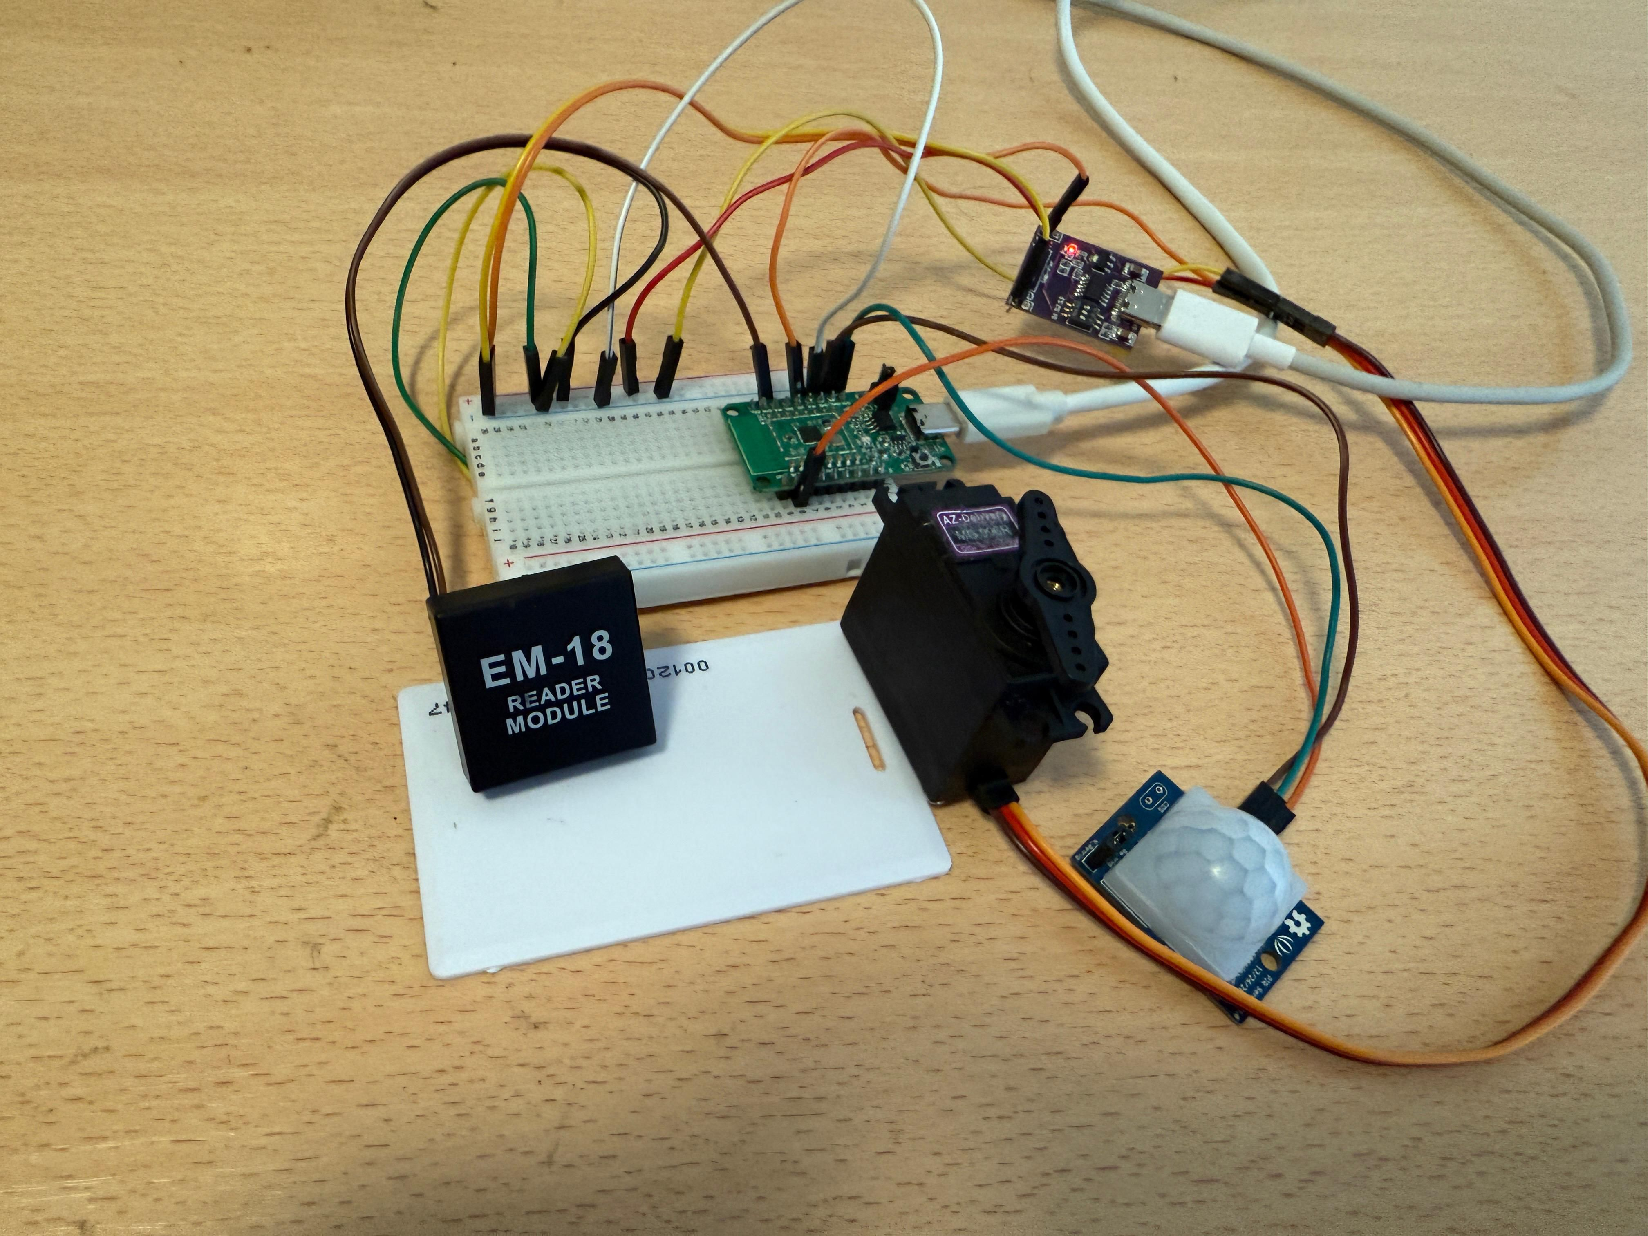
\includegraphics[width=0.7\textwidth]{comp.pdf}
    \caption{Components  showing the physical setup of the system.}
    \label{fig:comp}
    
\end{figure}
Figure~\ref{fig:comp} shows  hardware structure of the Smart Security Door Lock System. It consists of a PineCone BL602 microcontroller, an EM-18 RFID reader, a PIR motion sensor, an MG996R servo motor, and a Wi-Fi module. They are all to be run together in coordination for safe access control with RFID authentication and motion detection.

Besides, the system has a software level where users can communicate with the hardware using a mobile app. The users can view access logs remotely, receive alerts via motion detection, and control door access in real time using the app.



\subsection{Hardware Components}
\subsubsection{PineCone BL602}

Figure~\ref{fig:Pine} shows the PineCone BL602 microcontroller, which is the core microcontroller of the Smart Security Door Lock System, managing RFID authentication, motion detection, servo motor control, and Wi-Fi communication. It is a RISC-V-based, low-power IoT microcontroller designed for efficiency, featuring Wi-Fi 2.4 GHz, Bluetooth 5.0, UART, PWM, and GPIO interfaces, making it ideal for smart security applications \cite{BL602Datasheet}.

In this system, the EM-18 RFID reader \cite{EM18Datasheet} sends authentication data to the PineCone BL602 via UART (GPIO4 RX). If the tag matches a stored credential, the microcontroller activates the MG996R servo motor (GPIO17 PWM) \cite{MG996RServoMotor} to unlock the door. The PIR motion sensor (GPIO5) detects movement near the door and sends notifications through a Wi-Fi-enabled mobile app. The microcontroller operates in Access Point (AP) mode, allowing real-time remote monitoring and access control via predefined API endpoints.

\begin{figure}[H] % Use [H] to force the image placement
    \centering
    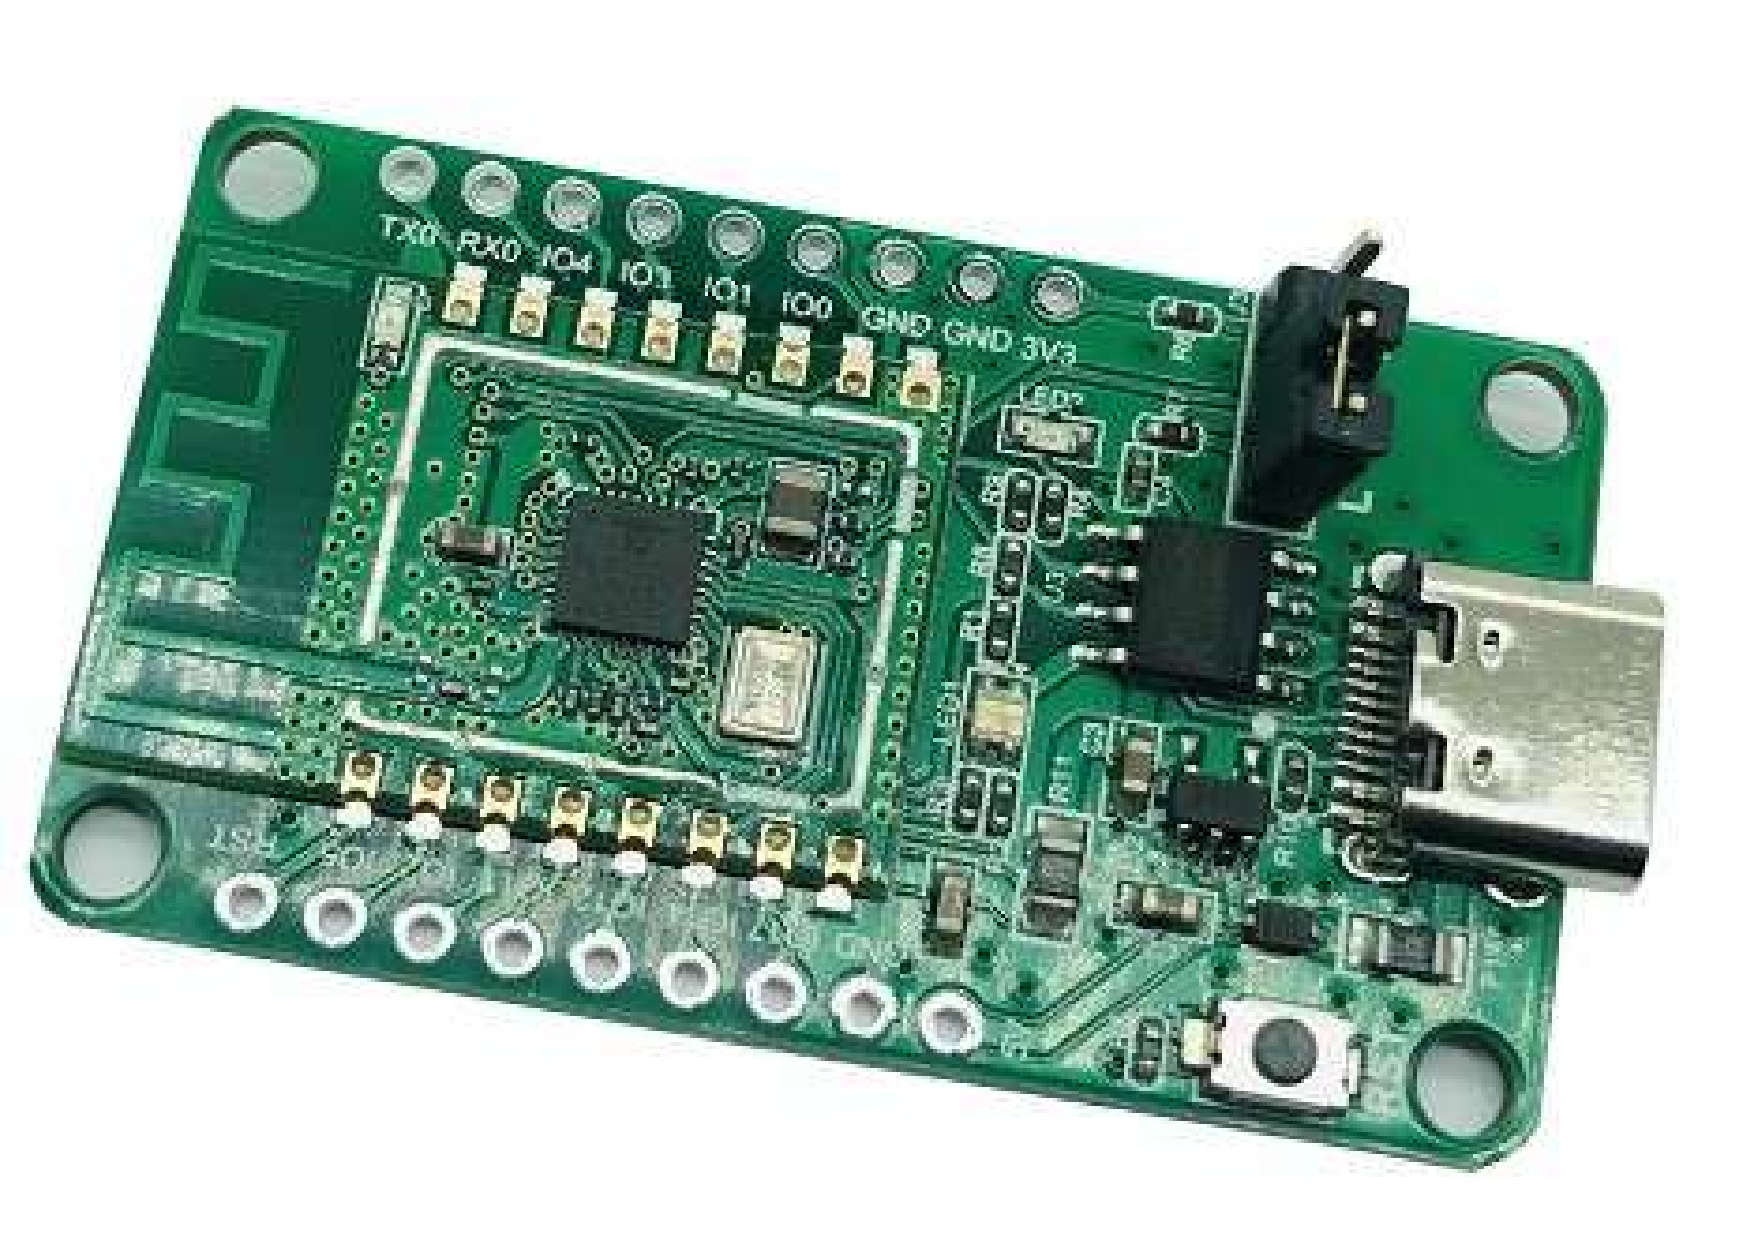
\includegraphics[width=0.6\textwidth]{Pine.pdf}
    \caption{PineCone BL602 microcontroller}
    \label{fig:Pine}
\end{figure}

With its low power consumption, built-in wireless connectivity, and multiple peripheral interfaces, the PineCone BL602 provides a cost-effective, scalable, and energy-efficient solution for IoT-based secure smart door access control \cite{BL602Datasheet}.




\subsubsection{EM-18 RFID Reader}

Figure~\ref{fig:em18} shows the EM-18 RFID Reader, which is one of the simplest components of the Smart Security Door Lock System and is used to identify users carrying RFID tags or cards. The reader, which operates at a frequency of 125 kHz, can identify RFID tags up to a maximum distance of 10 cm \cite{EM18Datasheet}. The module is widely used in security systems because it is power-efficient, fast, and easy to connect with microcontrollers \cite{RFIDReaderEM18}.

\begin{figure}[H] % Use [H] to force the image placement
    \centering
    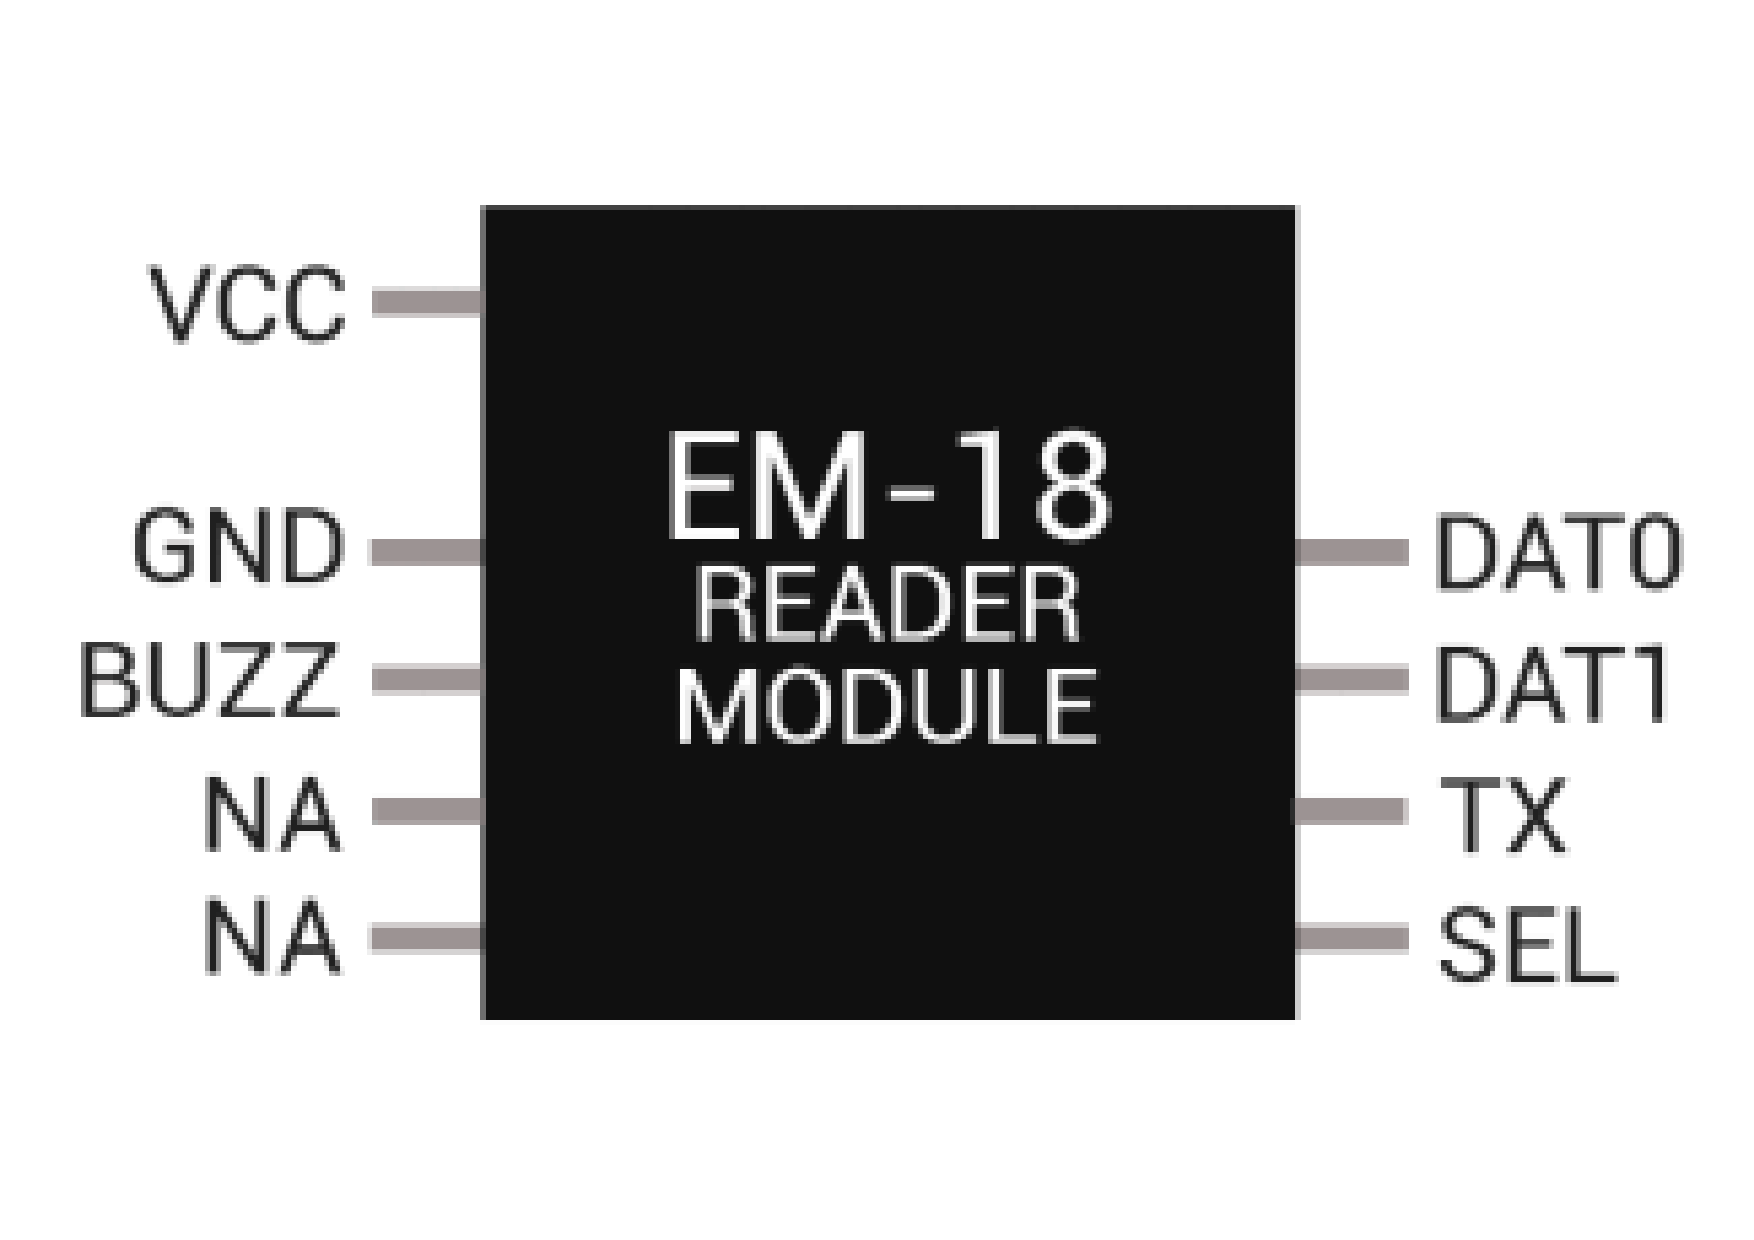
\includegraphics[width=0.7\textwidth]{em18.pdf}
    \caption{EM-18 RFID Reader}
    \label{fig:em18}
\end{figure}

Here, the EM-18 sends the data to the PineCone BL602 microcontroller using UART communication at 9600 bps \cite{UARTWiki}. As soon as the user approaches an RFID card to the reader, the reader identifies the tag ID and sends it to the microcontroller on its TX pin. The microcontroller authenticates if the tag is valid or not. If valid, the servo motor opens the door. In the event of an unauthorized tag, access is denied by the system, and the attempt is logged \cite{RFIDInc2025}.

The EM-18 consumes 5V power and supports Wiegand or UART mode, making it easy to integrate into IoT-based intelligent security systems \cite{EM-18}. Its compact size, reliability, and quick response make it an ideal choice for smart locks.


\subsubsection{PIR Motion Sensor}



Figure~\ref{fig:PIR} shows the PIR (Passive Infrared)\cite{PIRMotion} Motion Sensor is a critical unit of the Smart Security Door Lock System, used for detecting movement near the door and enhancing security. It is an infrared radiation from living organisms detecting unit, hence utilized effectively for motion sensing of humans. The sensor is widely used in security systems because of its low power usage, high reliability, and easy integration with microcontrollers.

Here, the PIR sensor is attached to the PineCone BL602 microcontroller on GPIO5. It continuously scans the environment for motion. When movement is detected, the sensor triggers the microcontroller to log the event and inform the mobile application. In contrast to the RFID reader, which manages door entrance, the PIR sensor is a secondary security component that checks for suspicious activity around the door.
\begin{figure}[H] % Use [H] to force the image placement
    \centering
    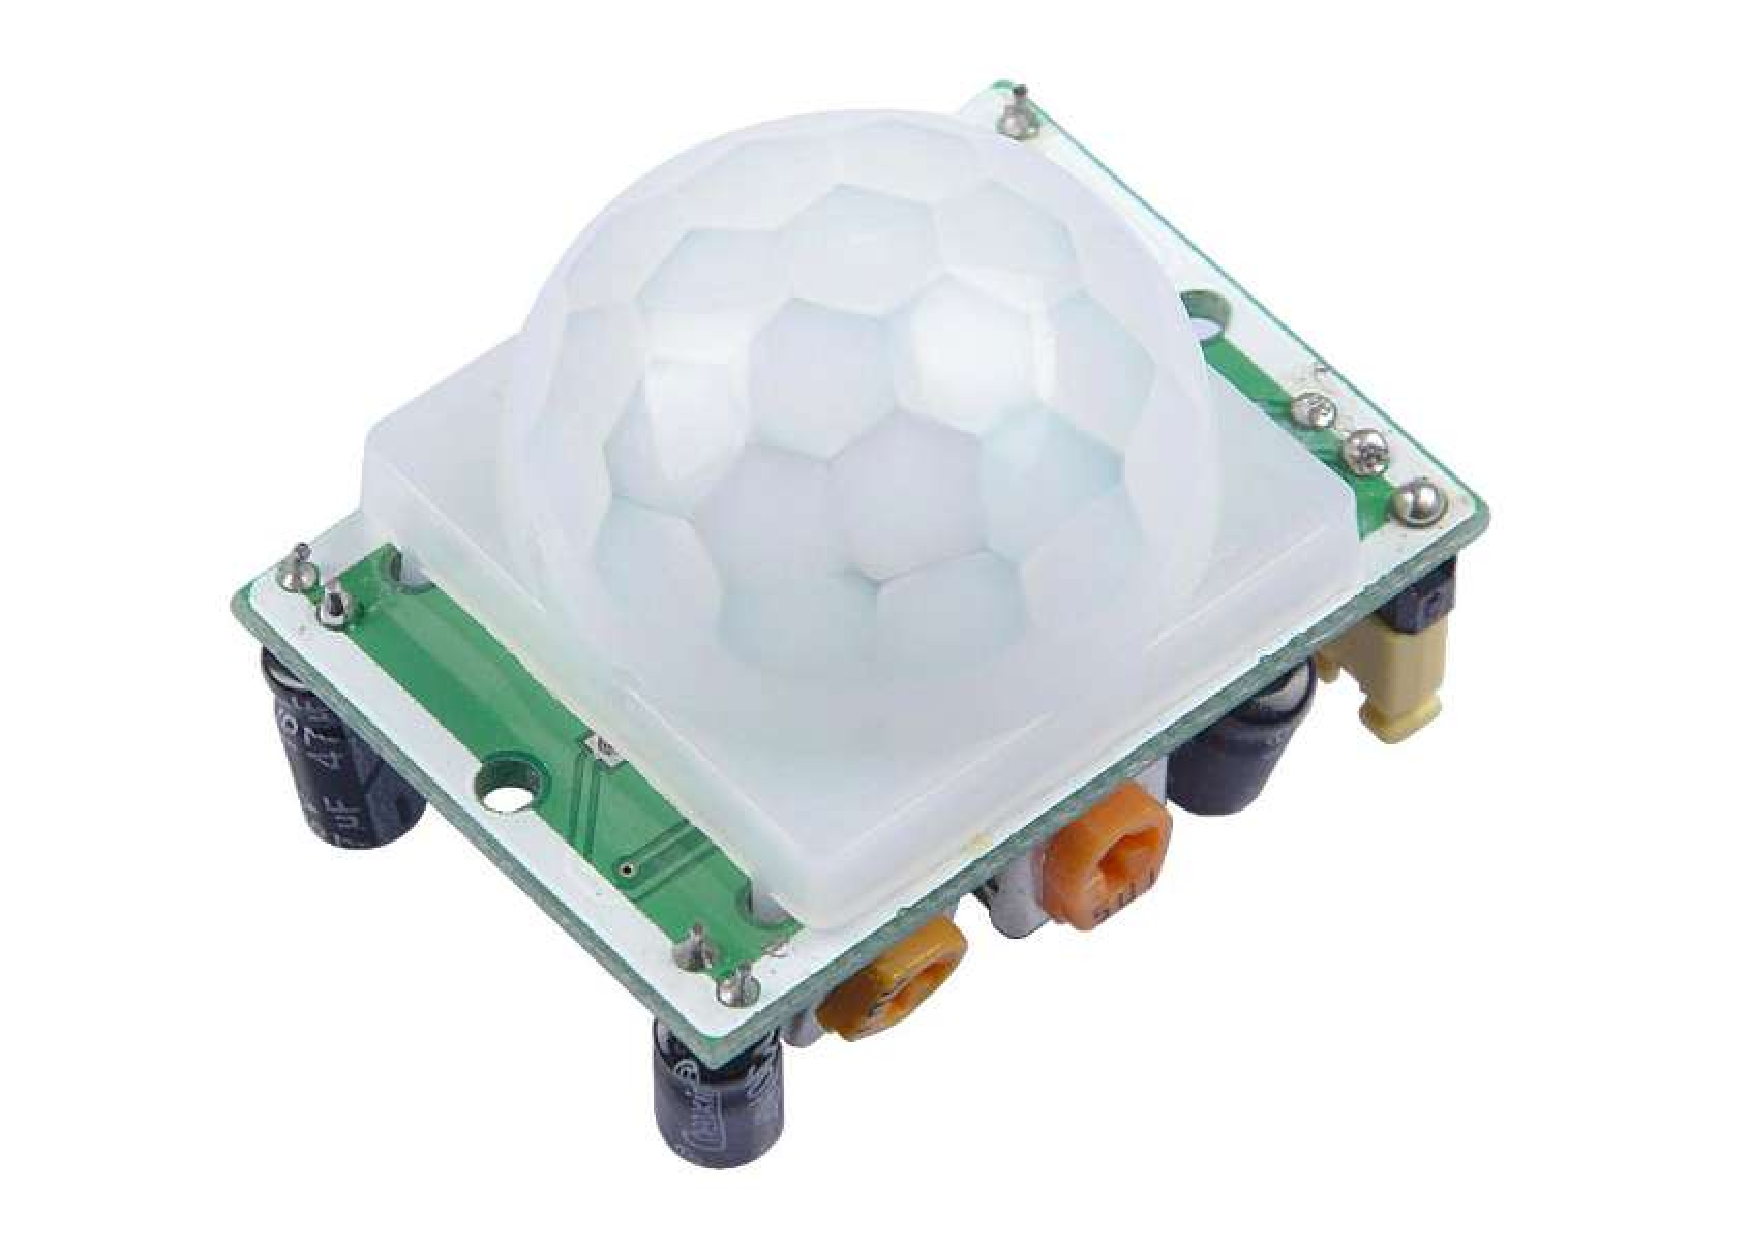
\includegraphics[width=0.5\textwidth]{PIR.pdf}
    \caption{PIR Motion Sensor}
    \label{fig:PIR}
\end{figure}
The sensor is powered by 3.3V to 5V voltage and is sensitive with adjustable delay time, which can be set as per environment requirements. The sensor consumes low power and offers high sensitivity and thus is fit for smart home security.


\subsubsection{Servo Motor (MG996R)}

\begin{figure}[H] % Use [H] to force the image placement
    \centering
    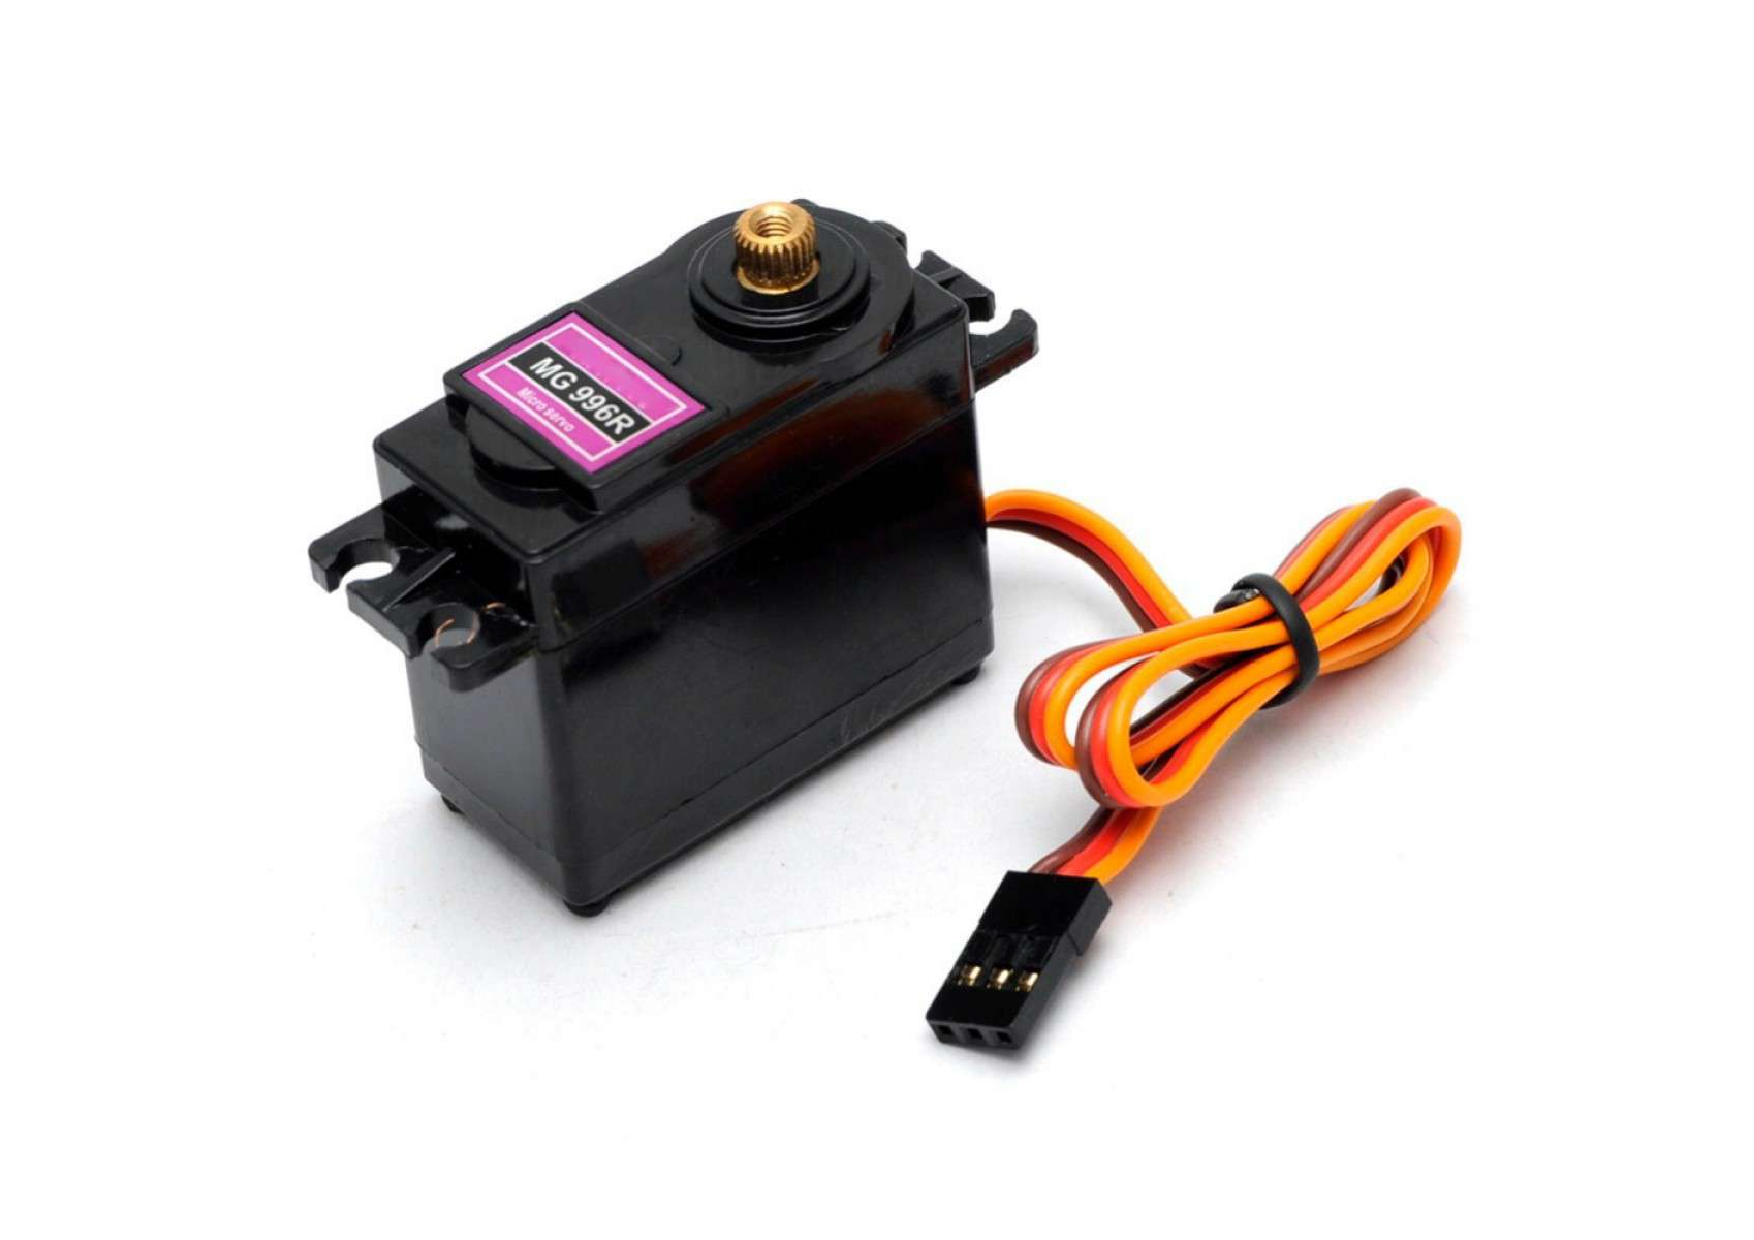
\includegraphics[width=0.5\textwidth]{motor.pdf}
    \caption{Servo Motor (MG996R)}
    \label{fig:motor}
\end{figure}

Figure~\ref{fig:motor} shows the MG996R Servo Motor, which is a vital part of the Smart Security Door Lock System as it drives the door lock and unlock process. It is a high-torque servo motor known for its accuracy, power, and fast response, making it best suited for use in smart security applications \cite{MG996RServoMotor}.

In this configuration, the servo motor is connected to the PineCone BL602 microcontroller using GPIO17, an extrnal power supply with 5V and controlled with PWM (Pulse Width Modulation) signals \cite{PWMGeeksforGeeks}. After presenting the RFID tag in front of the system, the microcontroller sends a PWM signal to the servo motor, causing it to rotate 90 degrees to unlock the door. After a short delay, the motor returns to its initial position, securing the door.

The MG996R operates at 5V, delivering high torque and stable performance. Its high sensitivity control and metal gearsensure a smooth and reliable locking mechanism. Due to its durability and precise movement, it is widely used in security applications requiring automated access control\cite{Patel2021}.


\subsubsection{RFID Tag}

Figure~\ref{fig:tag} shows the RFID \cite{RFIDWiki} Tag, which is the central module of the Smart Security Door Lock System and is used for storing and presenting a unique identification code in order to authenticate users. It operates at a frequency of 125 kHz in order to enable the EM-18 RFID reader to read and pick the ID of the tag remotely.

All RFID tags have a pre-programmed unique ID, which is stored in a microchip within the tag and sent when they are brought near the RFID reader. The ID is received and forwarded to the PineCone BL602 microcontroller by the EM-18 reader, which verifies whether the tag is being carried by an authenticated user. It allows entry if yes and denies entry if no.

\begin{figure}[H] % Use [H] to force the image placement
    \centering
    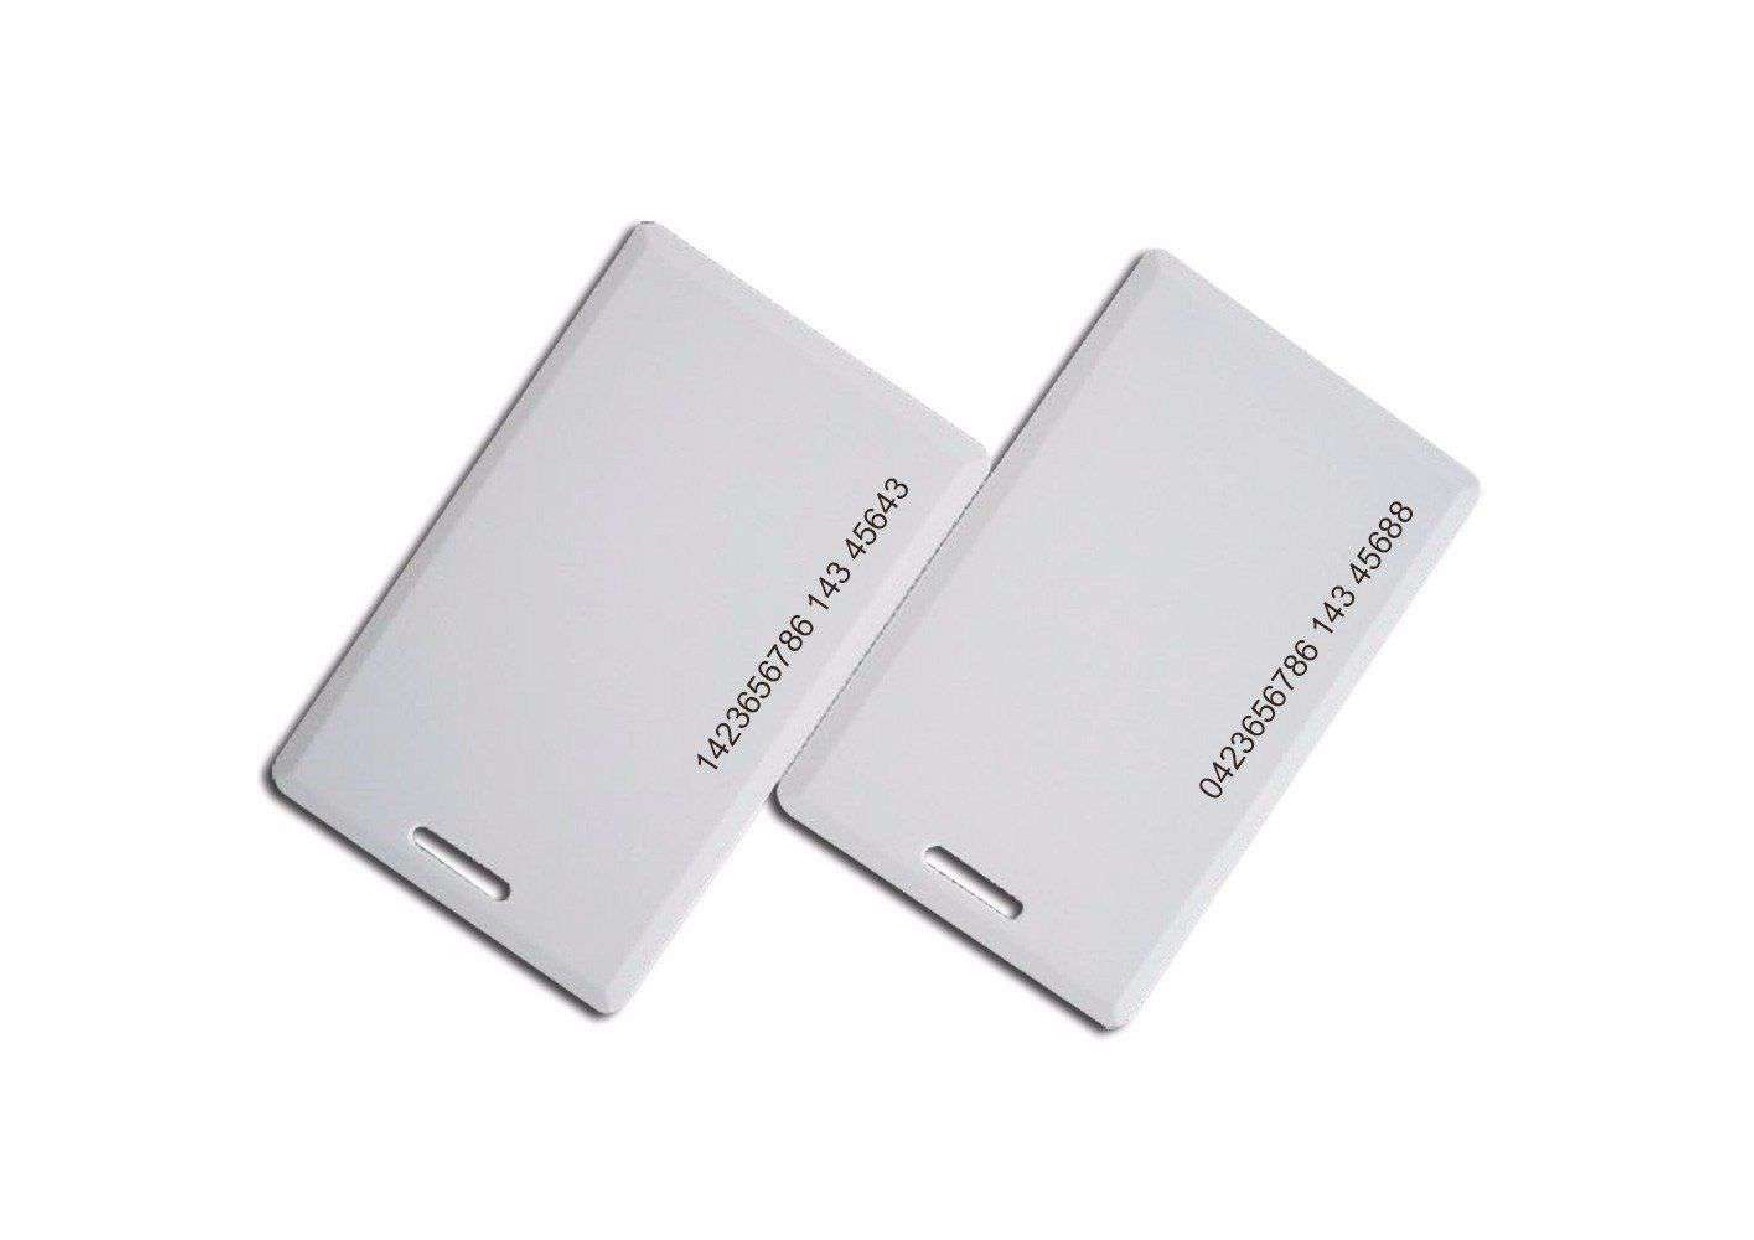
\includegraphics[width=0.5\textwidth]{tag.pdf}
    \caption{RFID Tag}
    \label{fig:tag}
\end{figure}

RFID tags are not battery-powered and therefore are highly rugged and low-maintenance. They are durable, small, and low-cost, making them highly suited for secure access control solutions to ensure instant, touchless authentication in smart security systems \cite{RFIDInc2025}.



\subsection{Hardware Configuration}
The Smart Security Door Lock System is built around the PineCone BL602 microcontroller, which serves as the central processing unit, interfacing with multiple peripherals, including an RFID module (EM-18), PIR motion sensor, servo motor, and power supply. These components work together to provide secure and automated access control. The system architecture ensures efficient communication between different modules while maintaining a reliable and low-power design. Proper hardware integration is crucial to achieving seamless operation, real-time authentication, and remote monitoring functionalities.
 
 \subsubsection{Pin Diagram} 
 \begin{figure}[H]
    \centering
    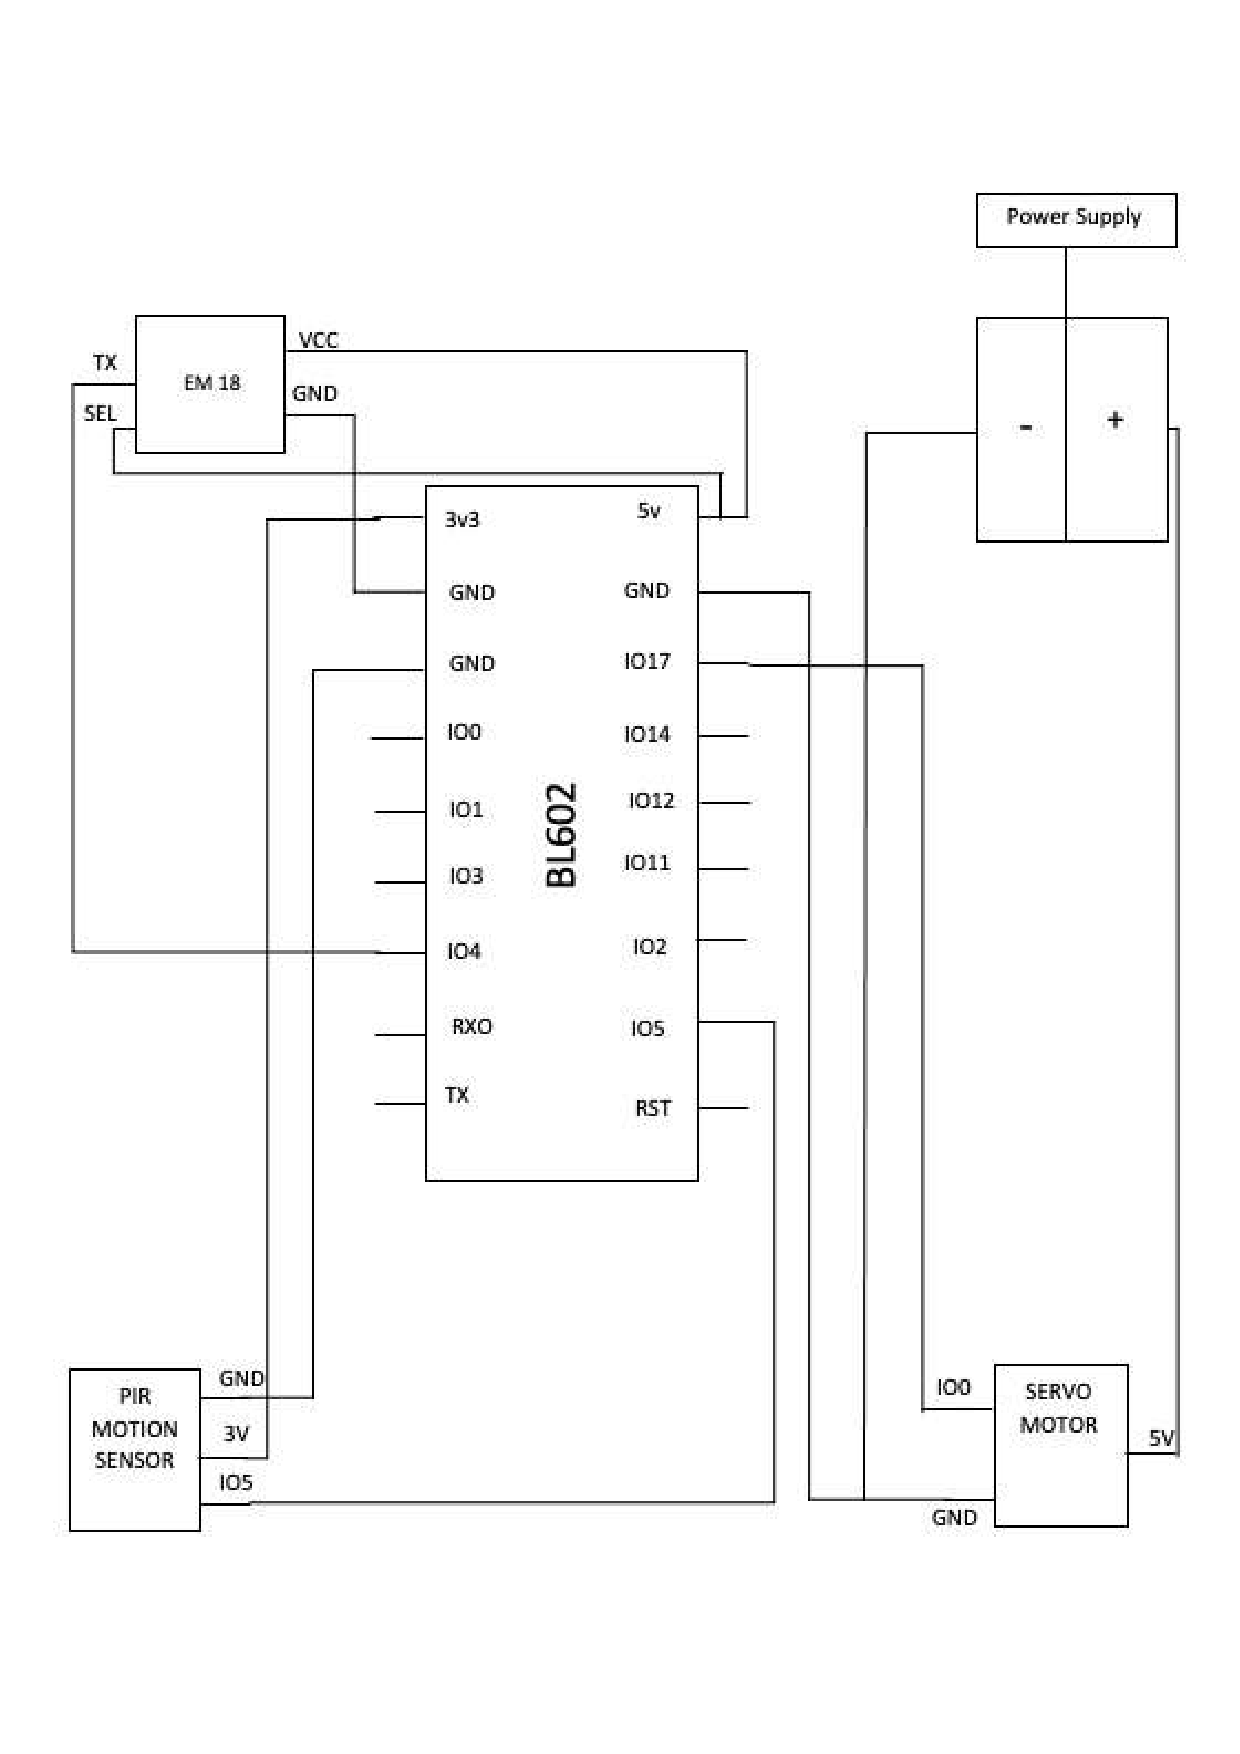
\includegraphics[width=0.75\textwidth]{pin.pdf}
    \caption{Pin Diagram showing the connection of components to the PineCone BL602 microcontroller.}
    \label{fig:pin}
\end{figure}
The complete pin configuration of the system is shown in Figure~\ref{fig:pin}, illustrating the GPIO mappings and power distribution. The diagram visually represents how the RFID reader, PIR sensor, servo motor, and power supply are connected to the BL602 microcontroller, ensuring proper communication and power management.

The PineCone BL602 microcontroller is at the heart of the system, managing data flow between various components. The RFID reader is connected via UART for secure authentication, while the PIR motion sensor provides motion detection input to trigger security alerts. The servo motor is controlled using PWM signals to automate the locking and unlocking mechanism. Each component is assigned specific GPIO pins to ensure efficient operation without interference.



\subsubsection{RFID Module (EM-18) Connections}
The RFID module is responsible for reading the RFID tag and sending the tag ID to the microcontroller for authentication. It plays a key role in access control, allowing only authorized users to unlock the door. The connections between the EM-18 module and the BL602 microcontroller are outlined in Table~\ref{tab:rfid_connections}, which details the corresponding pin mappings and their functions.


\begin{table}[H]
    \centering
    \begin{tabular}{|l|l|l|}
        \hline
        \textbf{RFID Module Pin} & \textbf{Connected to BL602 Pin} & \textbf{Function} \\
        \hline
        TX & RX0 & UART Data Transmission \\
        SEL & 5V & Selection Signal (Active Low) \\
        VCC & 5V & Power Supply (3.3V) \\
        GND & GND & Ground Connection \\
        \hline
    \end{tabular}
    \caption{Connections of RFID Module (EM-18) with BL602}
    \label{tab:rfid_connections}
\end{table}

\subsubsection{PIR Motion Sensor Connections}
The PIR motion sensor detects movement near the door and alerts the microcontroller. It provides an additional layer of security by notifying users about any suspicious activity. The connections for the PIR sensor are outlined in Table~\ref{tab:pir_connections}, which details the specific pin mappings and their respective functions.


\begin{table}[H]
    \centering
    \begin{tabular}{|l|l|l|}
        \hline
        \textbf{PIR Sensor Pin} & \textbf{Connected to BL602 Pin} & \textbf{Function} \\
        \hline
        3V & 3V3 & Power Supply (3.3V) \\
        IO5 & IO5 & Motion Detection Signal \\
        GND & GND & Ground Connection \\
        \hline
    \end{tabular}
    \caption{Connections of PIR Motion Sensor with BL602}
    \label{tab:pir_connections}
\end{table}

\subsubsection{Servo Motor (MG996R) Connections}
The servo motor controls door locking and unlocking. Its connections with the microcontroller are shown in Table~\ref{tab:servo_connections}.


\begin{table}[H]
    \centering
    \begin{tabular}{|l|l|l|}
        \hline
        \textbf{Servo Pin} & \textbf{Connected to BL602 Pin} & \textbf{Function} \\
        \hline
        Signal (PWM) & IO0 & Door Lock/Unlock Control \\
        VCC & 5V & Power Supply (5V) \\
        GND & GND & Ground Connection \\
        \hline
    \end{tabular}
    \caption{Connections of Servo Motor (MG996R) with BL602}
    \label{tab:servo_connections}
\end{table}

\subsubsection{Power Supply Connections}
The power supply ensures stable power distribution across all components, providing the necessary voltage levels for efficient system operation. The connections are detailed in Table~\ref{tab:power_connections}.


\begin{table}[H]
    \centering
    \begin{tabular}{|l|l|l|}
        \hline
        \textbf{Power Supply Pin} & \textbf{Connected to BL602 Pin} & \textbf{Function} \\
        \hline
        +5V & 5V & Main System Power \\
        - (Ground) & GND & Common Ground \\
        \hline
    \end{tabular}
    \caption{Power Supply Connections}
    \label{tab:power_connections}
\end{table}


\subsection{Software Components}
The Smart Security Door Lock System is powered by embedded firmware and a mobile application, ensuring seamless communication between hardware components and users. The firmware for the \textbf{PineCone BL602 microcontroller} was developed using \textbf{Buffalo Lab's BL\_IOT\_SDK,} an open-source Software Development Kit (SDK) designed for IoT applications. This SDK provided pre-built libraries and APIs, enabling the implementation of RFID authentication, motion detection, servo motor control, and Wi-Fi communication. Using C-based programming \cite{CDevDocs}, the firmware was flashed onto the microcontroller, ensuring real-time processing and secure access control.

We followed the guide \cite{BLFlashEnv} to gain a thorough understanding of the fundamentals of program development and deployment on PineCone BL602.

For firmware flashing and configuration, Dev Cube, a tool provided by Bouffalo Lab, was used. It allowed for MCU programming, RF performance testing, and system configuration, ensuring stability and optimized functionality. Users can monitor and control the security system through a mobile application developed in Android Studio (Java) \cite{JavaOracleDocs} \cite{AndroidStudio}. The app provides real-time access logs, motion detection alerts, and remote unlocking functionality via Wi-Fi communication with the microcontroller.

Predefined API endpoints retrieve authentication and motion logs, ensuring instant security updates. The mobile app offers an intuitive interface for managing door access, allowing users to track entry records and delete unnecessary logs. Additionally, the mobile app integrates push notifications, ensuring that users receive instant security alerts in case of unauthorized access attempts or motion detection events. The application also features a simple and user-friendly design, making it accessible to users of all technical backgrounds. This integration of firmware and mobile software delivers a secure, efficient, and user-friendly smart security solution.




\subsection{Software Implementation}
The Smart Security Door Lock System is designed to be functional in its entirety by integrating embedded firmware, wireless networking, and a mobile app. The software handles RFID authentication, motion detection, servo motor control, and Wi-Fi remote access in order to create an efficient and secure user experience. The core of the software relies on the PineCone BL602 microcontroller, written in C language in the BL\_IOT\_SDK platform, which provides precompiled libraries for communication, peripheral control, and IoT connection. Firmware consists of different modules, each handling distinct functionalities within the system.

Firmware is made up of several significant C files, each responsible for different aspects of the system. The main.c file acts as the control center and is responsible for system components initialization and managing their interaction. Proper communication between the RFID reader, motion sensor, servo motor, and Wi-Fi module is ensured by this file. RFID authentication is controlled in the rfid.c file, which uses UART communication (GPIO4 RX0) to read tag IDs from the EM-18 RFID Reader. This module processes the incoming ID, compares it with a predefined database, and provides a response signal to grant or deny access. The motion.c file manages motion detection through the PIR Motion Sensor (attached to GPIO5). It runs continuously in the background and notifies the system when motion is detected, logging unauthorized attempts at entry.

The servo.c file drives the servo motor, which controls the locking and unlocking mechanism of the door. It accepts authentication signals from the RFID module and powers the MG996R Servo Motor using GPIO17, utilizing PWM \cite{PWMGeeksforGeeks} (Pulse Width Modulation) signals for precise movement. Upon successful authentication, the servo motor rotates 90 degrees to open the door and then returns to its original position after a short delay. The wifi.c module enables wireless connectivity, allowing the system to communicate with a remote mobile application. It sets up an HTTP server on the BL602, through which users can retrieve real-time access logs, receive motion detection notifications, and remotely control the door.

Each hardware component is interfaced directly with the PineCone BL602 microcontroller through the following pin configurations:

\begin{itemize}
    \item EM-18 RFID Reader is interfaced with UART, where its TX (Data Output) is connected to GPIO4 RX0. This connection allows rfid.c to read tag data and verify its authenticity.
    \item PIR Motion Sensor is connected to GPIO5 and is processed in motion.c, using an interrupt-based strategy to detect movement effectively.
    \item MG996R Servo Motor is controlled by PWM signals sent via GPIO17, allowing for precise motion to lock and unlock the door. This function is implemented in servo.c.
    \item Wi-Fi Module is integrated within BL602 and managed in wifi.c to enable secure wireless communication between the microcontroller and the mobile application.
\end{itemize}

The mobile application, developed using Android Studio (Java), provides an intuitive interface for interacting with the system. It communicates with the BL602 via Wi-Fi, enabling users to monitor access logs, receive motion detection alerts, and remotely unlock the door. To facilitate seamless communication, the firmware provides predefined API endpoints, which include:

\begin{itemize}
    \item /doorstatus.html – Retrieves access logs to display previous entries.
    \item /motion.html – Provides real-time motion detection status.
    \item /clearmotion.html – Clears older motion detection logs from the system.
\end{itemize}

By utilizing these API endpoints, the mobile application ensures real-time security notifications without interruptions. The system is optimized for efficiency, handling real-time authentication and event logging while maintaining low power consumption.

This integration of embedded firmware, mobile application, and wireless communication results in a robust and scalable smart security system. The structured approach guarantees secure authentication, real-time alerts, and remote monitoring capabilities, making it an efficient, reliable, and user-friendly solution for smart home security.

\begin{figure}[h]
    \centering
    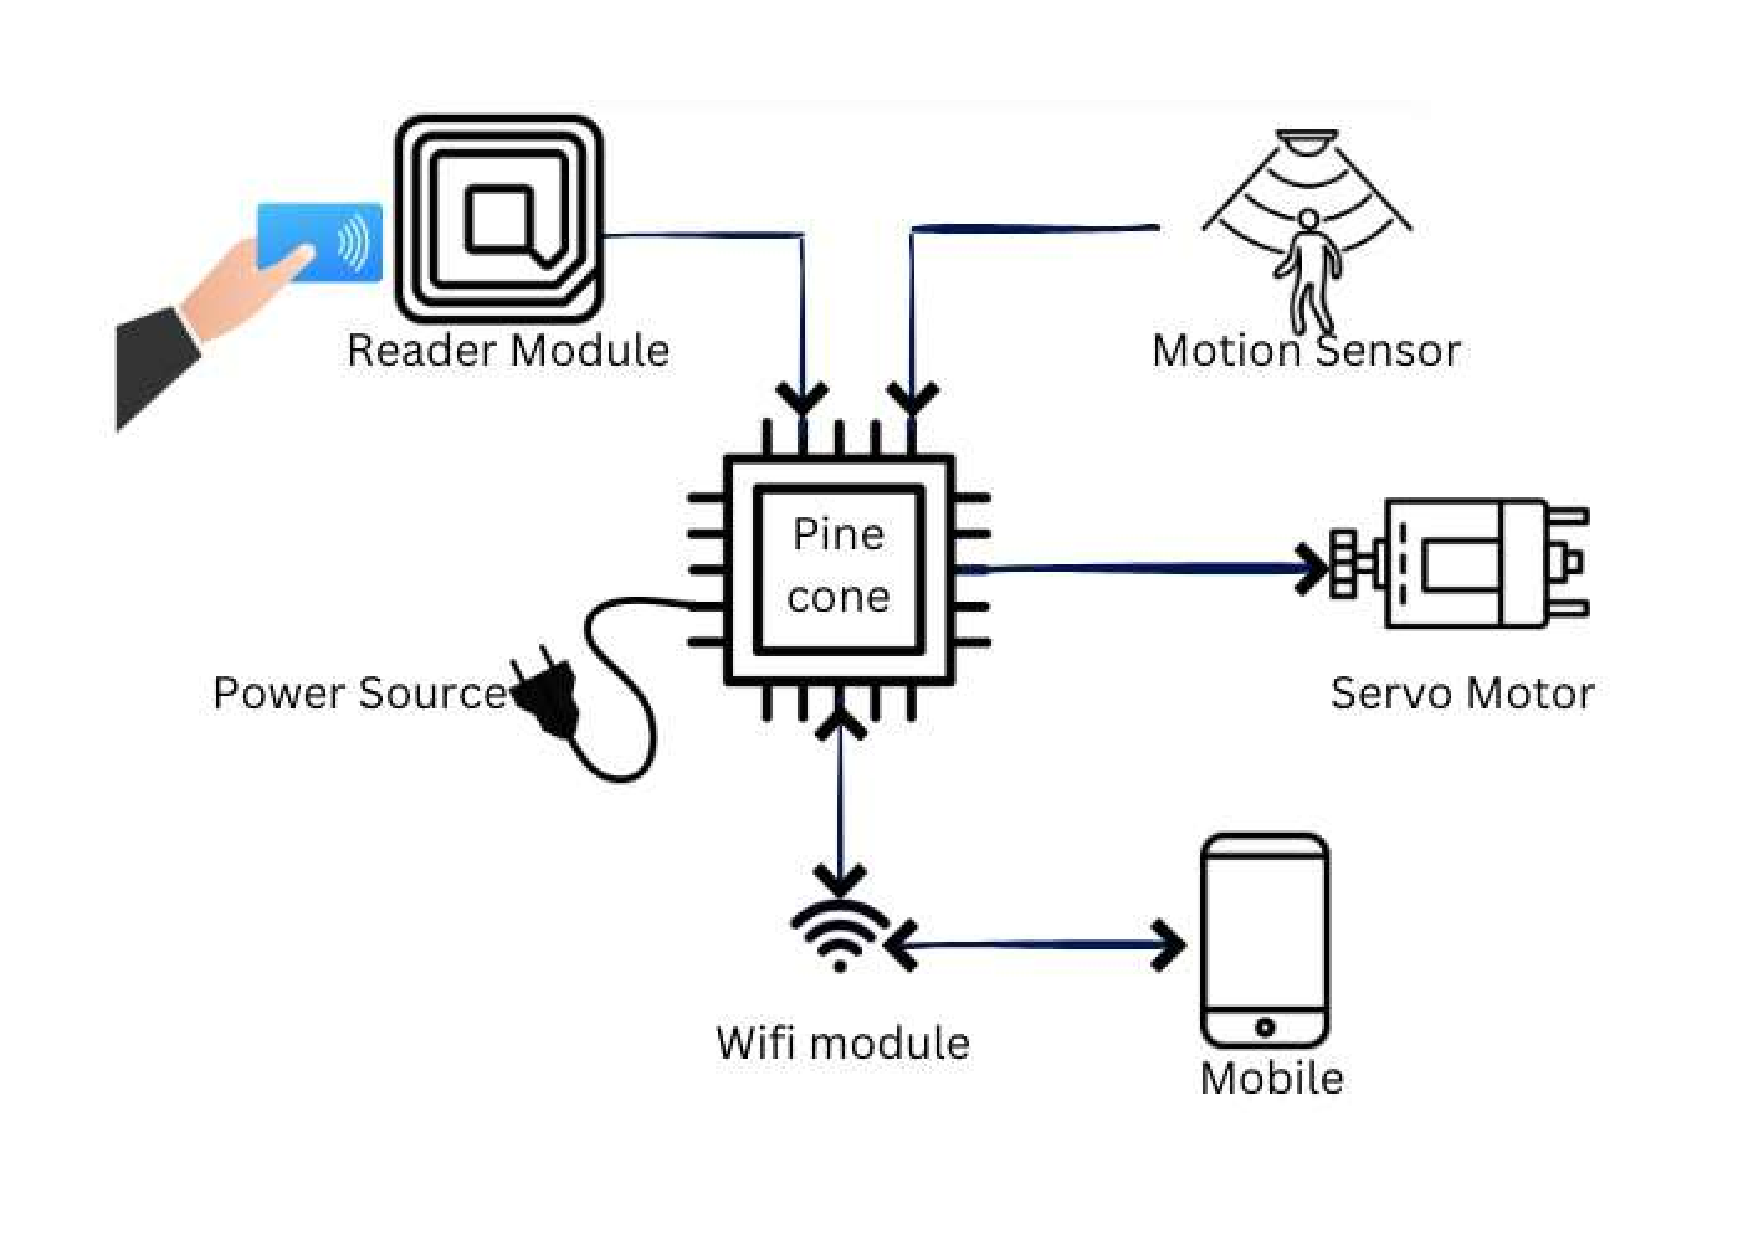
\includegraphics[width=0.7\textwidth]{dfd.pdf}
    \caption{Data Flow diagram}
    \label{fig:dfd}
\end{figure}

The system's operation is streamlined, as shown in Figure \ref{fig:dfd}. When an RFID card is scanned using the EM-18 RFID Reader, the scanned data is sent to the PineCone BL602 microcontroller through UART communication. The firmware processes the ID, verifies the user against a predefined database, and sends a notification to the mobile application. If the RFID tag is authorized, the person's name is displayed on the mobile app, and the servo motor is activated to unlock the door.

Additionally, the PIR Motion Sensor, connected to the PineCone BL602, continuously detects movement near the entrance. If motion is detected, an alert is triggered, and a notification is sent to the mobile application in real-time. This feature enhances security by allowing users to monitor unauthorized movements.

The Wi-Fi module on the BL602 facilitates communication between the microcontroller and the mobile app. The firmware hosts a set of API endpoints, which allow the mobile app to retrieve access logs, check the motion detection status, and remotely control the door lock.

The mobile application, developed using Android Studio (Java), provides users with an intuitive interface to track who accessed the door and when, as well as to receive real-time security notifications. Users can also view previous access logs and manually clear motion detection logs if necessary. This seamless integration between hardware, firmware, and mobile software ensures an efficient, secure, and user-friendly smart security solution.


The source code for this project is available on \textbf{\href{https://github.com/JOSHUAPBIJU/Smart-Door-Lock-System-based-on-IOT}{GitHub}} \cite{GitHubRepo2025}.


\section{Results}
\label{sec:results} 
Our System has been successfully deployed and tested. The system effectively monitors access control, motion detection, and remote control through a mobile app. Combining RFID authentication, motion detection, and Wi-Fi communication, the system provides secure real-time monitoring to users.

When tested, the system properly identified legitimate RFID tags to provide access and energize the servo motor to open the door. The invalid RFID attempts were denied access, and the system logged the event and sent a message to the mobile application. The motion sensor detected movement near the door, triggering alarms on the mobile application. The real-time updates keep users informed of access attempts and security events in real time.

The system was tested under different conditions, including testing multiple tags, testing for unauthorized access, and triggering the PIR motion sensor under different light conditions. The time taken between reading an RFID tag and door unlock was measured to be in milliseconds, ensuring smoothness. Additionally, motion detection alarms were successfully received via the mobile app in seconds, ensuring the real-time functionality of the system.

The Wi-Fi module allowed remote monitoring, and users could check access logs and motion notifications via the Android app. Connectivity testing confirmed that the system was responsive in a timely fashion within a local network environment, with a low-latency response to commands issued via the mobile app.

Overall, the Smart Security Door Lock System performed as desired to enable quick authentication, secure access control, and real-time monitoring. The verification tests confirmed that the system operated stably, and future improvements could provide further security, extend connectivity, and minimize power consumption.


\subsection{Sensor Testing}

The Smart Security Door Lock System incorporates motion detection, RFID authentication, and access logging to enhance security. Motion sensors detect movement near the door, while RFID ensures only authorized users gain access. Each access attempt is logged, and users receive real-time alerts via the mobile app. The following figures demonstrate system responses to motion detection, successful authentication, and unauthorized access attempts.


Figure~\ref{fig:detection} shows very clearly how the Passive Infrared (PIR) motion detector operates to detect motion by the door. The sensor is continuously monitoring the surroundings, constantly searching for a shift in infrared radiation as a result of movement. With each movement, the sensor generates a signal to update the system to deliver real-time security monitoring. The system instantaneously reacts by displaying the phrase "Motion detected" on the console, indicating that movement has been captured. Conversely, if there is no movement, "No motion" appears on the console, ensuring that the room remains untouched. Such real-time alerts allow the system to remain on guard round the clock, enhancing security by instantly detecting any intruder.
\begin{figure}[H]
    \centering
    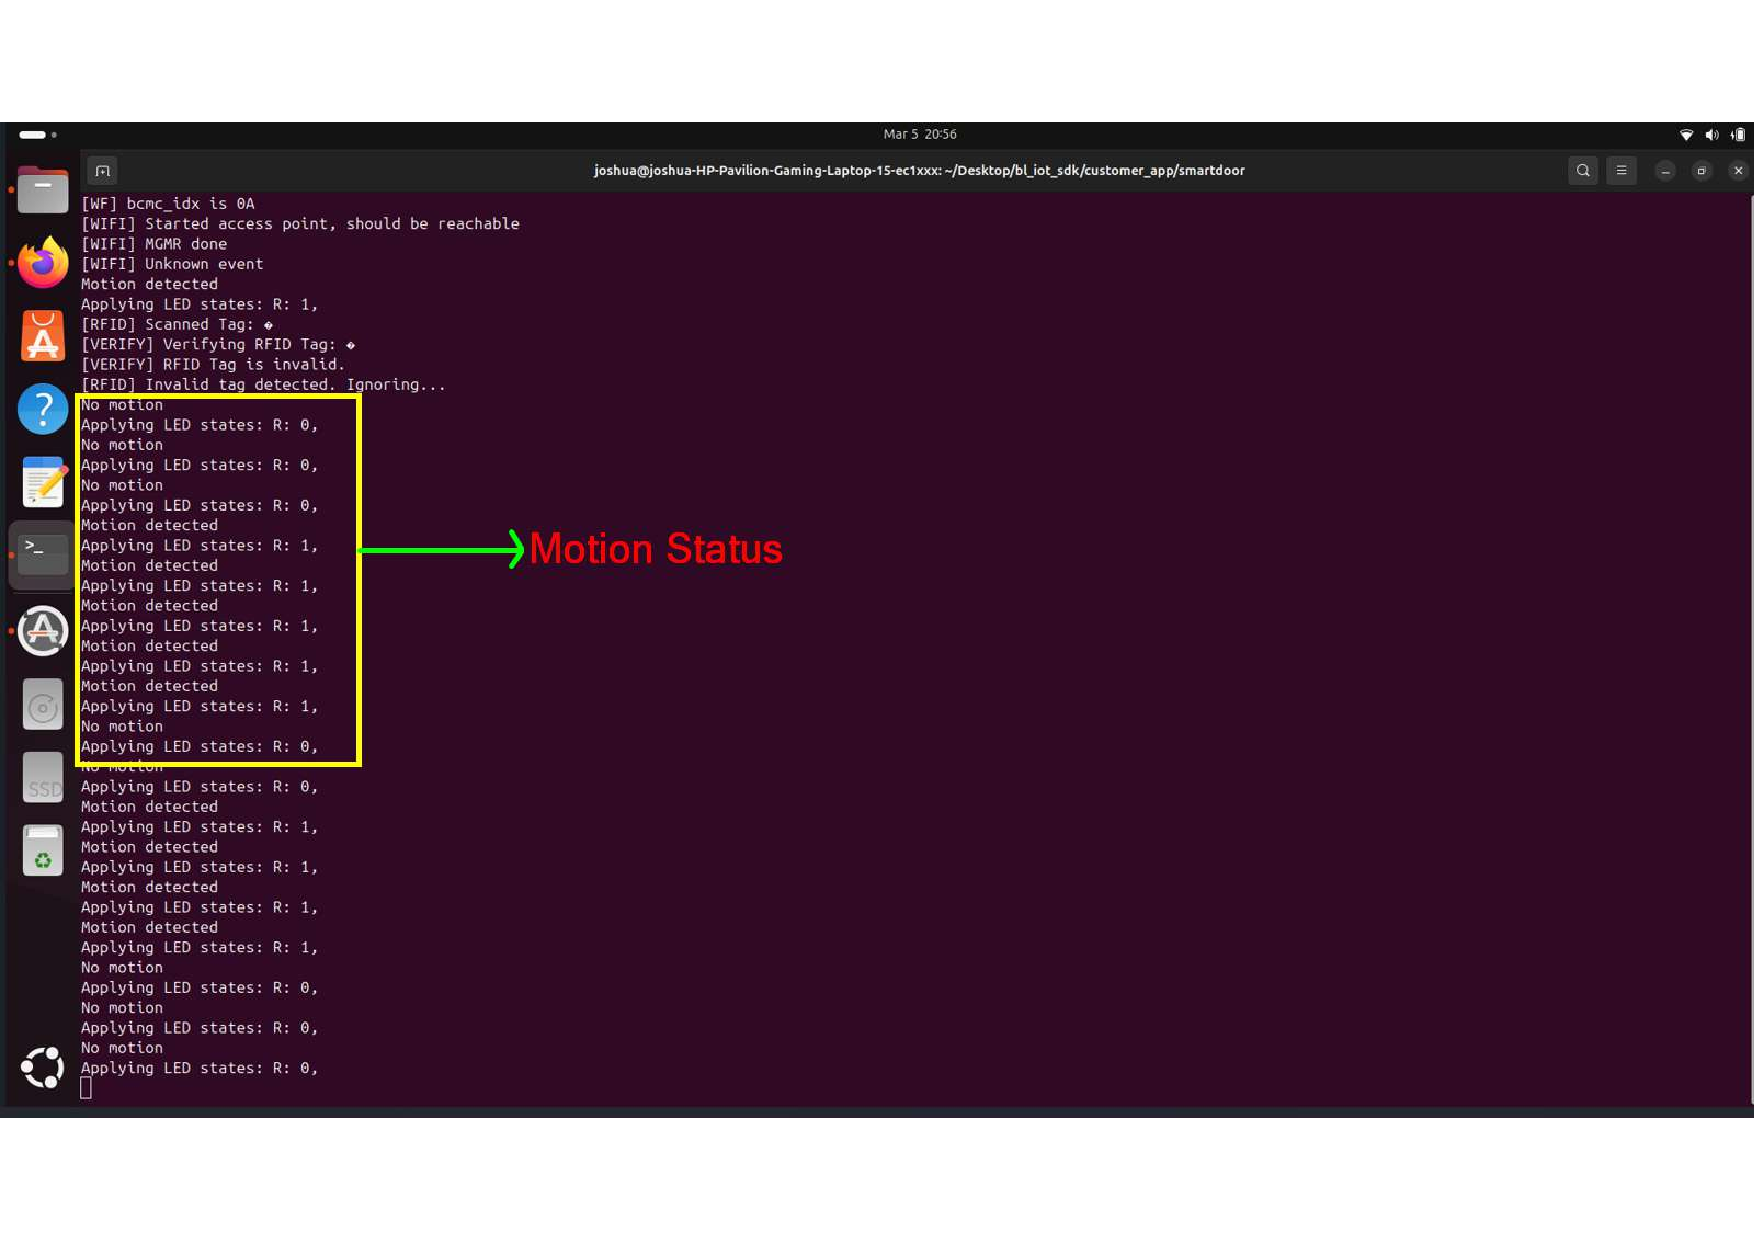
\includegraphics[width=0.71\textwidth]{motiondetection.pdf}
    \caption{Motion detection}
    \label{fig:detection}
\end{figure}

Figure~\ref{fig:action} illustrates the process of a effective authentication technique employing RFID technology. RFID tag reading of established integrity, its validity is verified via the system with a cross-referencing function from saved credentials. When the tag is recognized as authenticated, the system executes a set of actions: it powers up the servo motor to open the door, logs the attempt to access for auditing, and shows console messages to confirm that the authentication has been successful. The console prints messages such as "RFID Tag is valid" and "Valid tag detected", "Enabling servo motor," which explicitly indicate that access is granted. This simple process ensures access to only the permitted, in an efficient and secure way.

Figure~\ref{fig:invalidaction} illustrates an unauthorized RFID scan. When an invalid tag is detected, the system denies access, logs the failed attempt, and alerts the user. The console prints "RFID Tag is invalid" and "Unauthorized attempt detected", "Access denied". The door remains locked, and the mobile app receives a real-time security notification.



\begin{figure}[H]
    \centering
    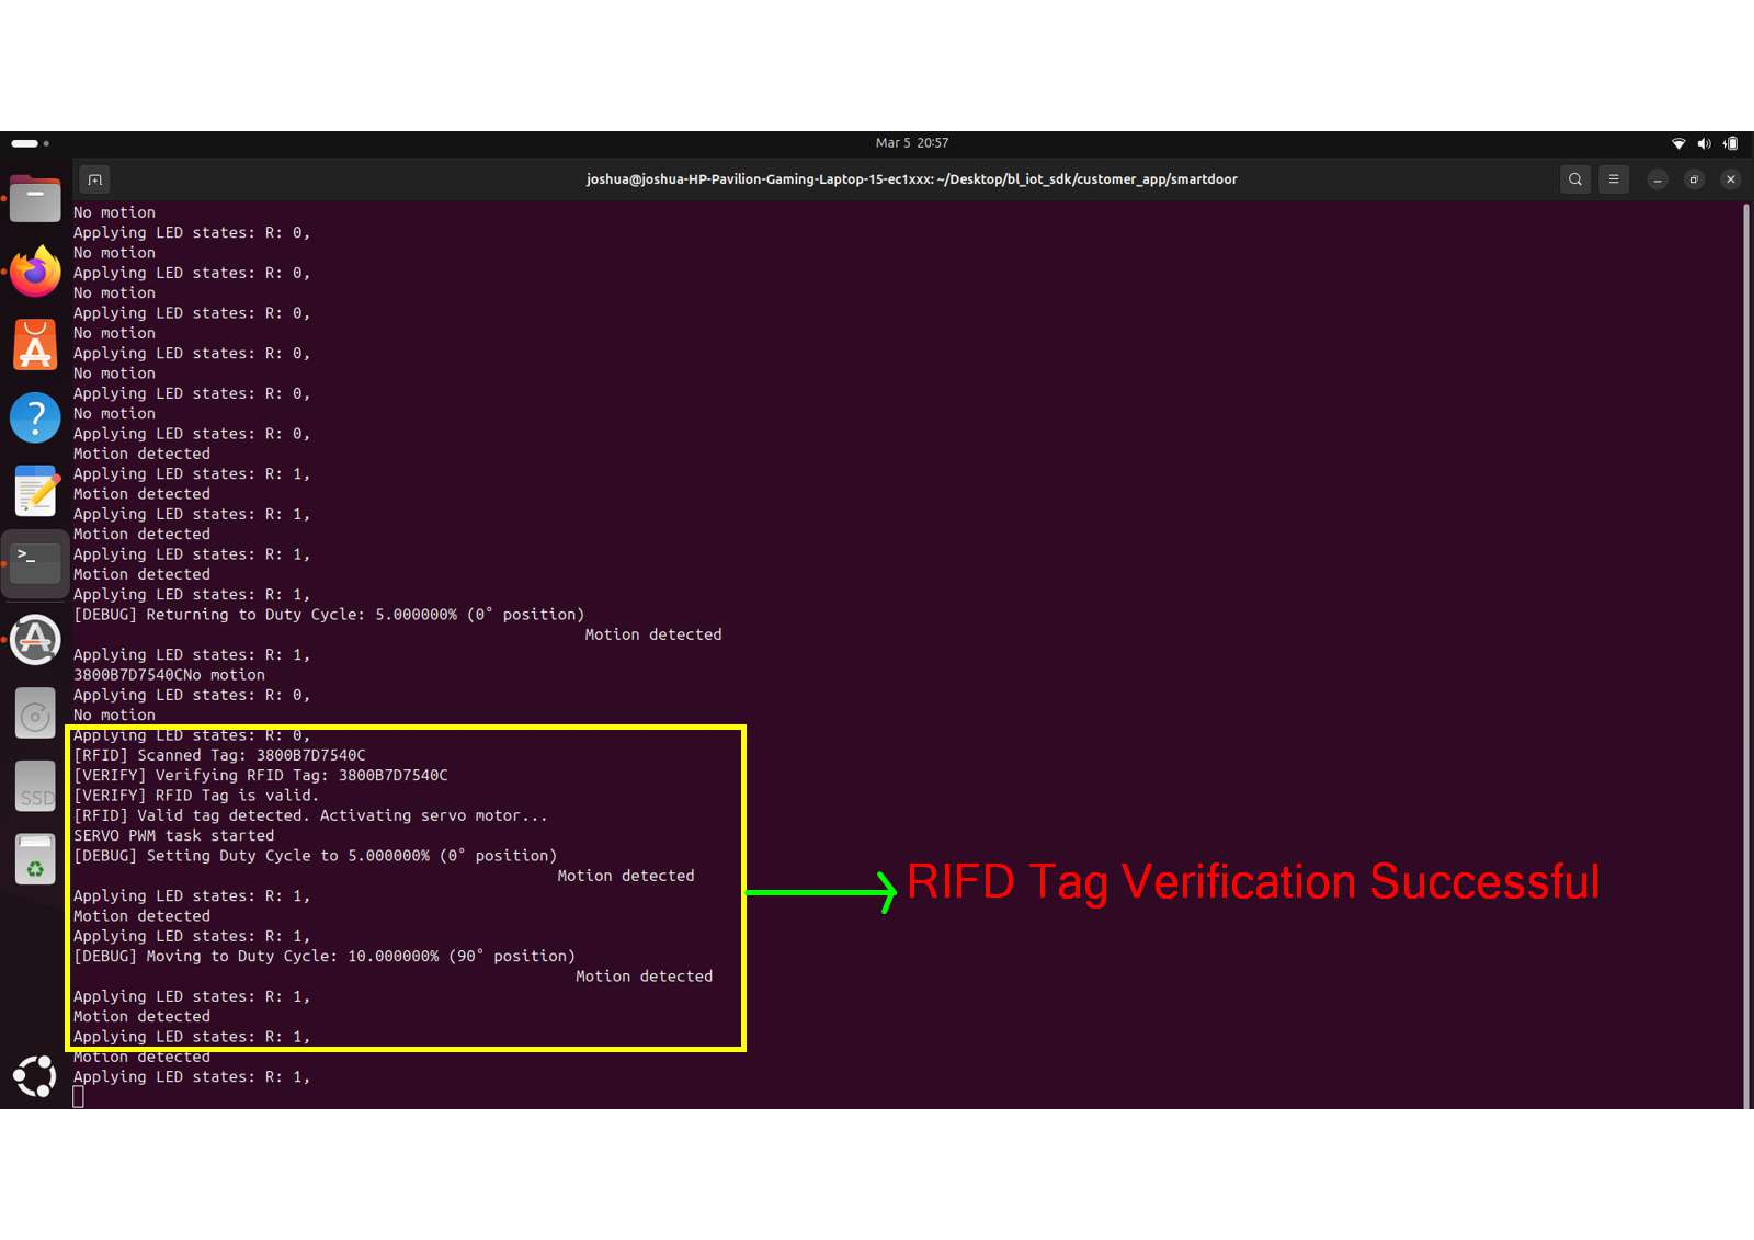
\includegraphics[width=0.72\textwidth]{motoraction.pdf}
    \caption{Verifying the tag and turning on the servo motor to open the door}
    \label{fig:action}
\end{figure}

\begin{figure}[H]
    \centering
    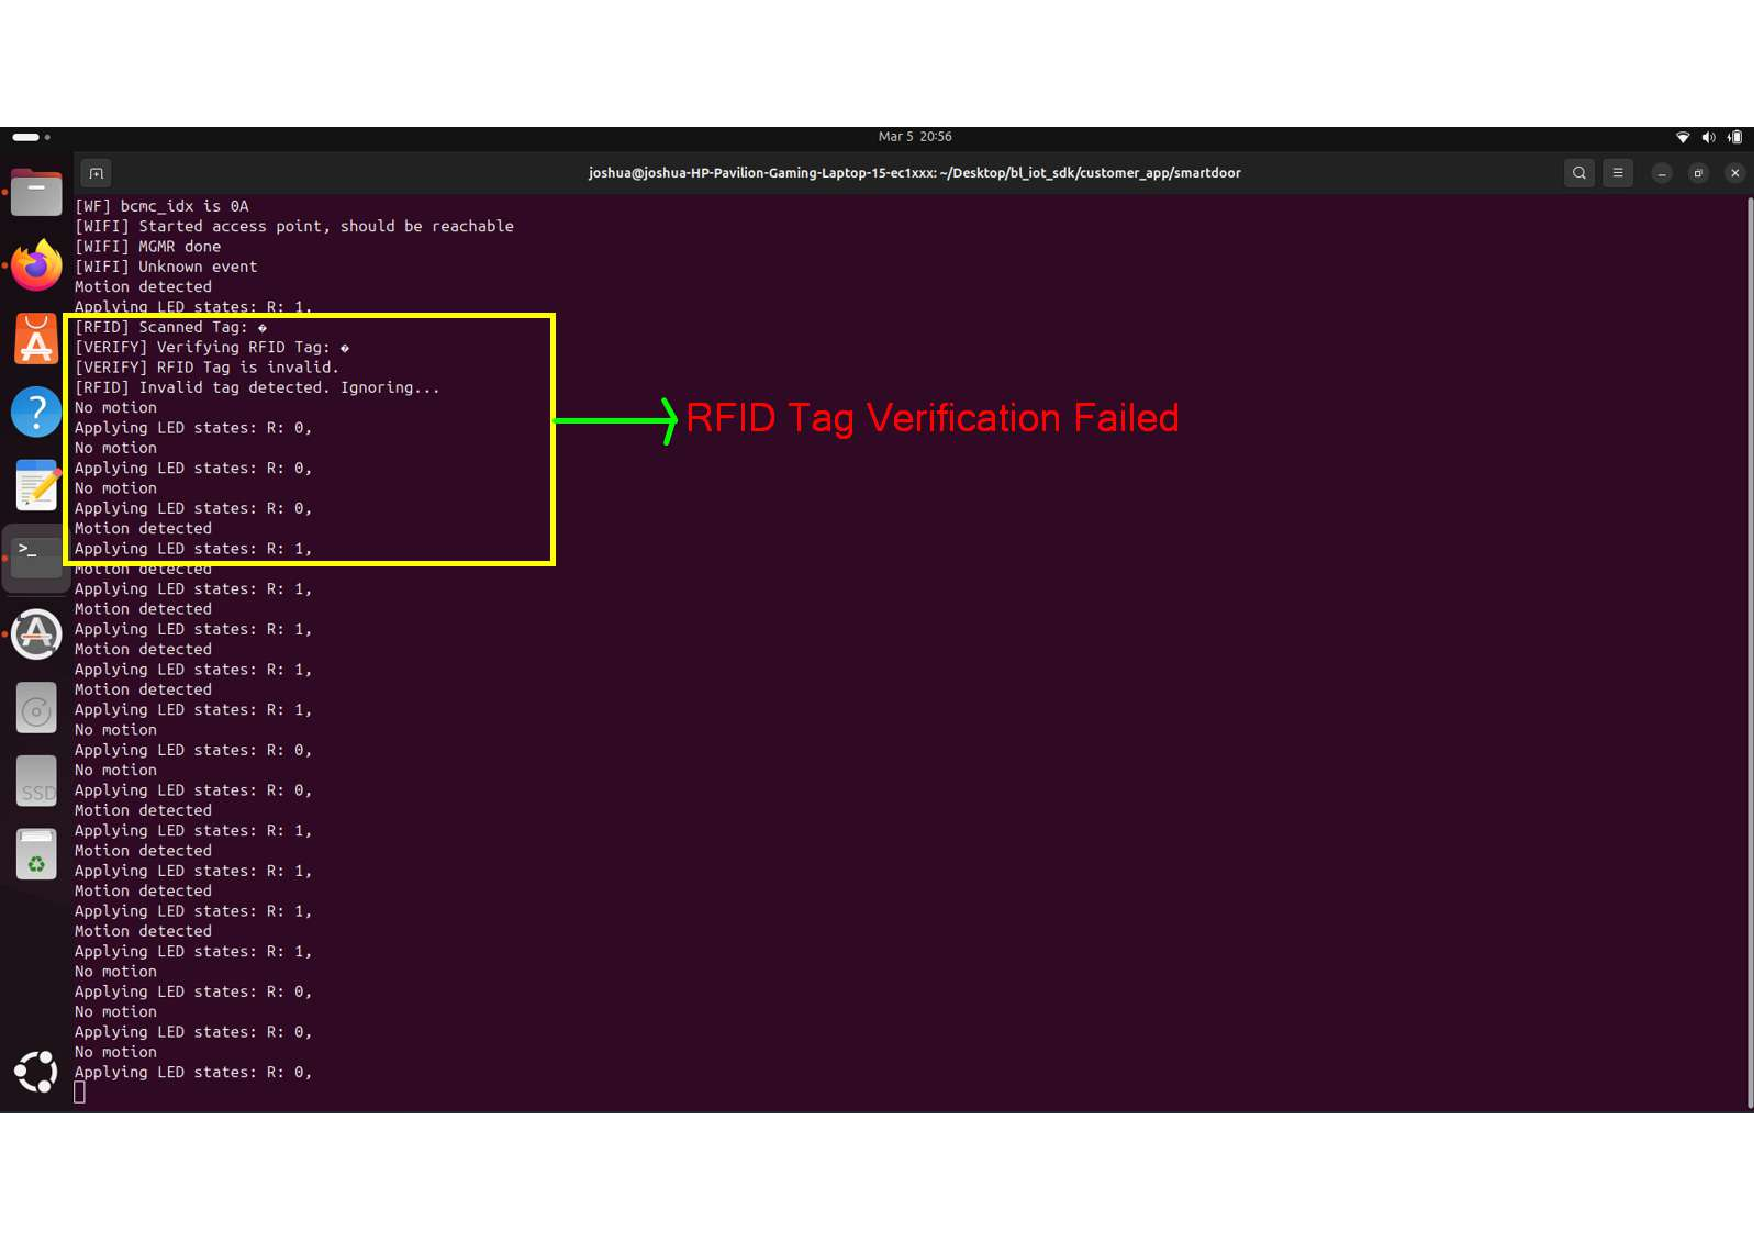
\includegraphics[width=0.72\textwidth]{inmotoraction.pdf}
    \caption{Invalid RFID scan attempt and system response}
    \label{fig:invalidaction}
\end{figure}





\subsection{Testing Results}

The Smart Security Door Lock System was tested under different conditions to validate sensor responses and real-time notifications appropriately.

Figure~\ref{fig:homepage} shows the mobile application's homepage, which serves as the user interface for monitoring and controlling the system. Figure~\ref{fig:notification} demonstrates the alert system, where the user is notified upon motion detection or an RFID scan. 

Figure~\ref{fig:user} depicts an instance where a valid user scans an authorized RFID tag, successfully unlocking the door. The mobile application displays the user ID of the last scanned tag and allows remote door control. Figure~\ref{fig:unknown} illustrates an unauthorized access attempt where an unregistered RFID tag is scanned. The system denies entry, logs the attempt, and marks the user ID as "Unknown" while notifying the user.
\subsection{Software Testing}
\label{sec:testing}
Software testing ensured the Smart Security Door Lock System functions reliably. Unit tests verified that RFID authentication correctly granted access while blocking unauthorized attempts. The motion sensor was tested for accurate detection, and the servo motor was evaluated for proper response.

The mobile application, developed in Android Studio (Java), was tested for real-time updates, notifications, and remote access. Wi-Fi connectivity was assessed to ensure seamless communication between the PineCone BL602 and the app. With the door open button, we can open the door remotely when connected to the same Wi-Fi. The app also includes a clear motion logs button to delete motion log data and an exit button to close the application.

All tests confirmed efficient system operation, delivering secure access control with accurate notifications. Below are the results of mode testing under different sensor conditions.





\begin{figure}[h]
    \centering
    \begin{minipage}{0.45\textwidth}
        \centering
        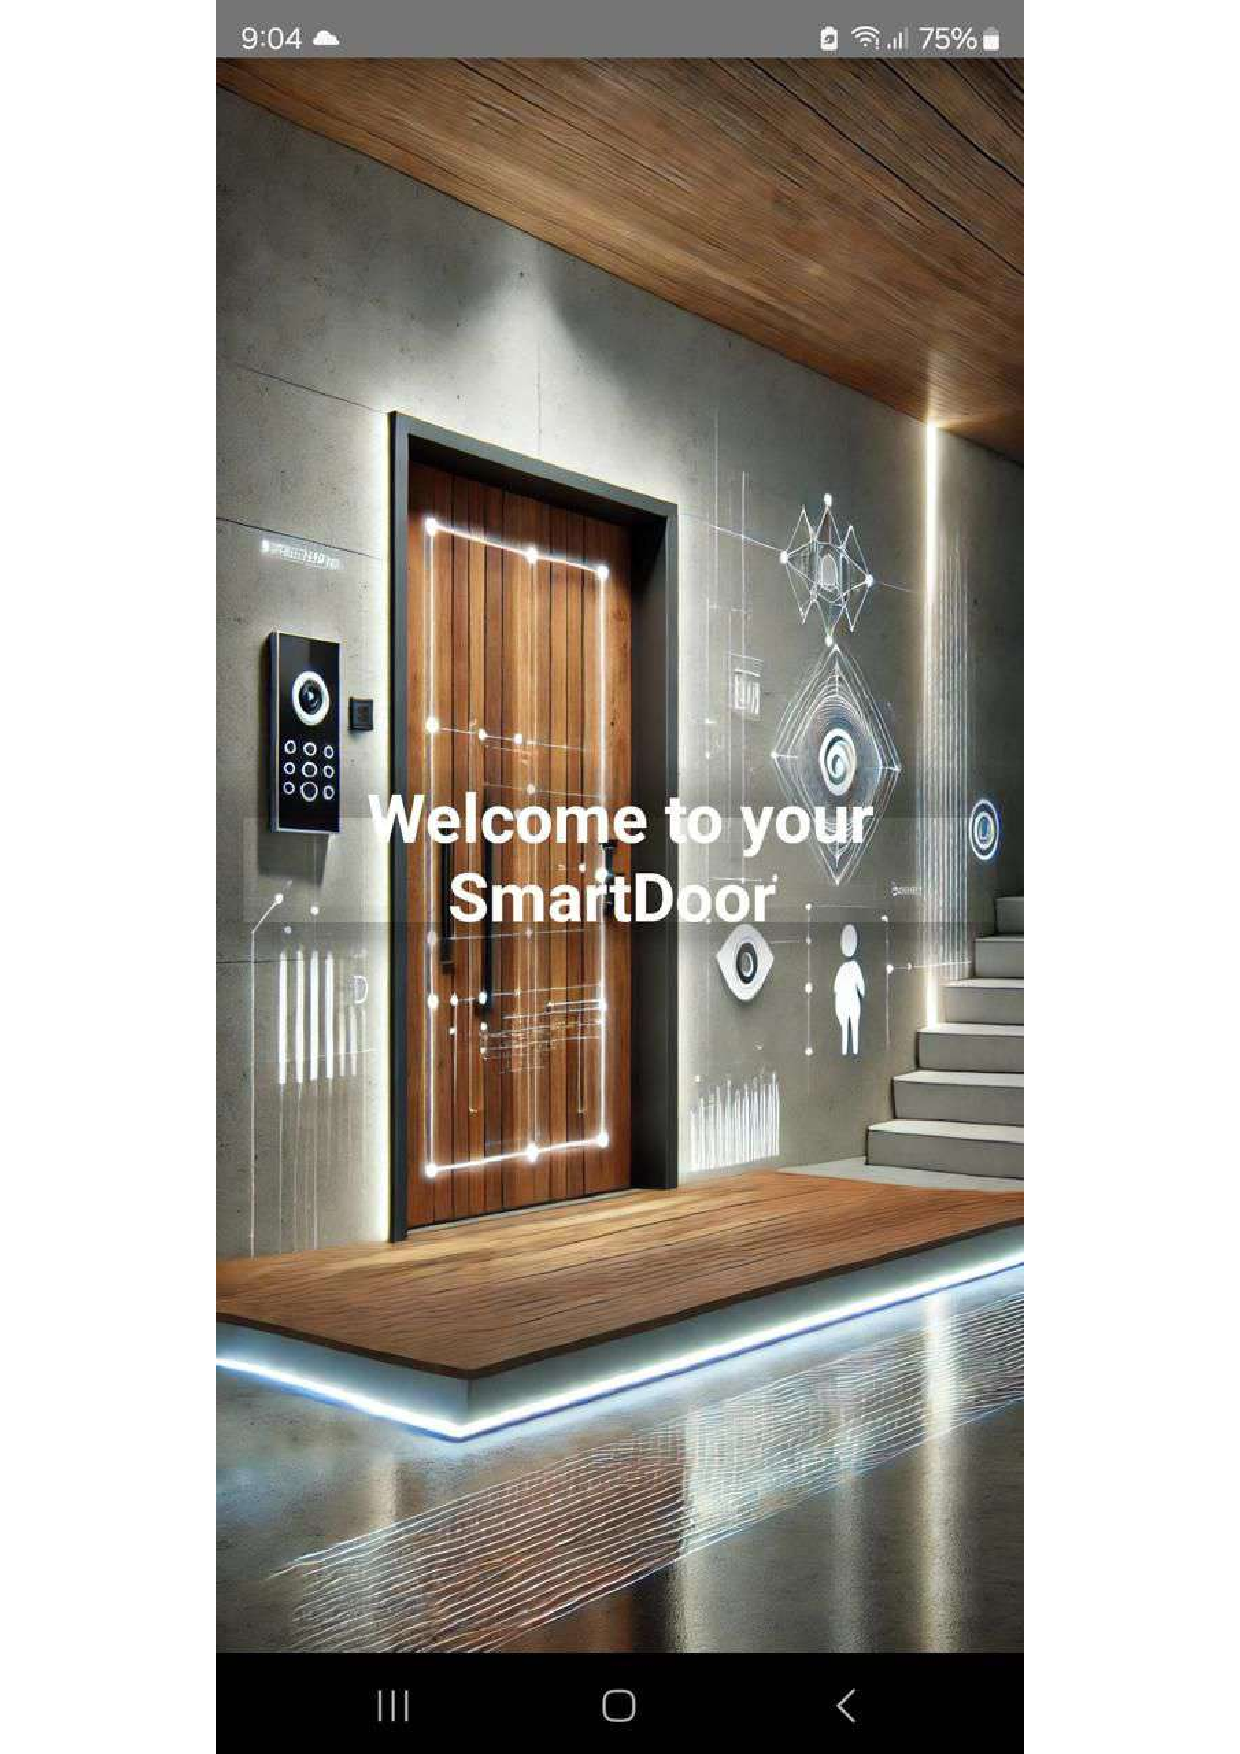
\includegraphics[width=0.9\textwidth]{homepage.pdf}
        \caption{Homepage of the mobile application}
        \label{fig:homepage}
    \end{minipage}
    \hfill
    \begin{minipage}{0.45\textwidth}
        \centering
        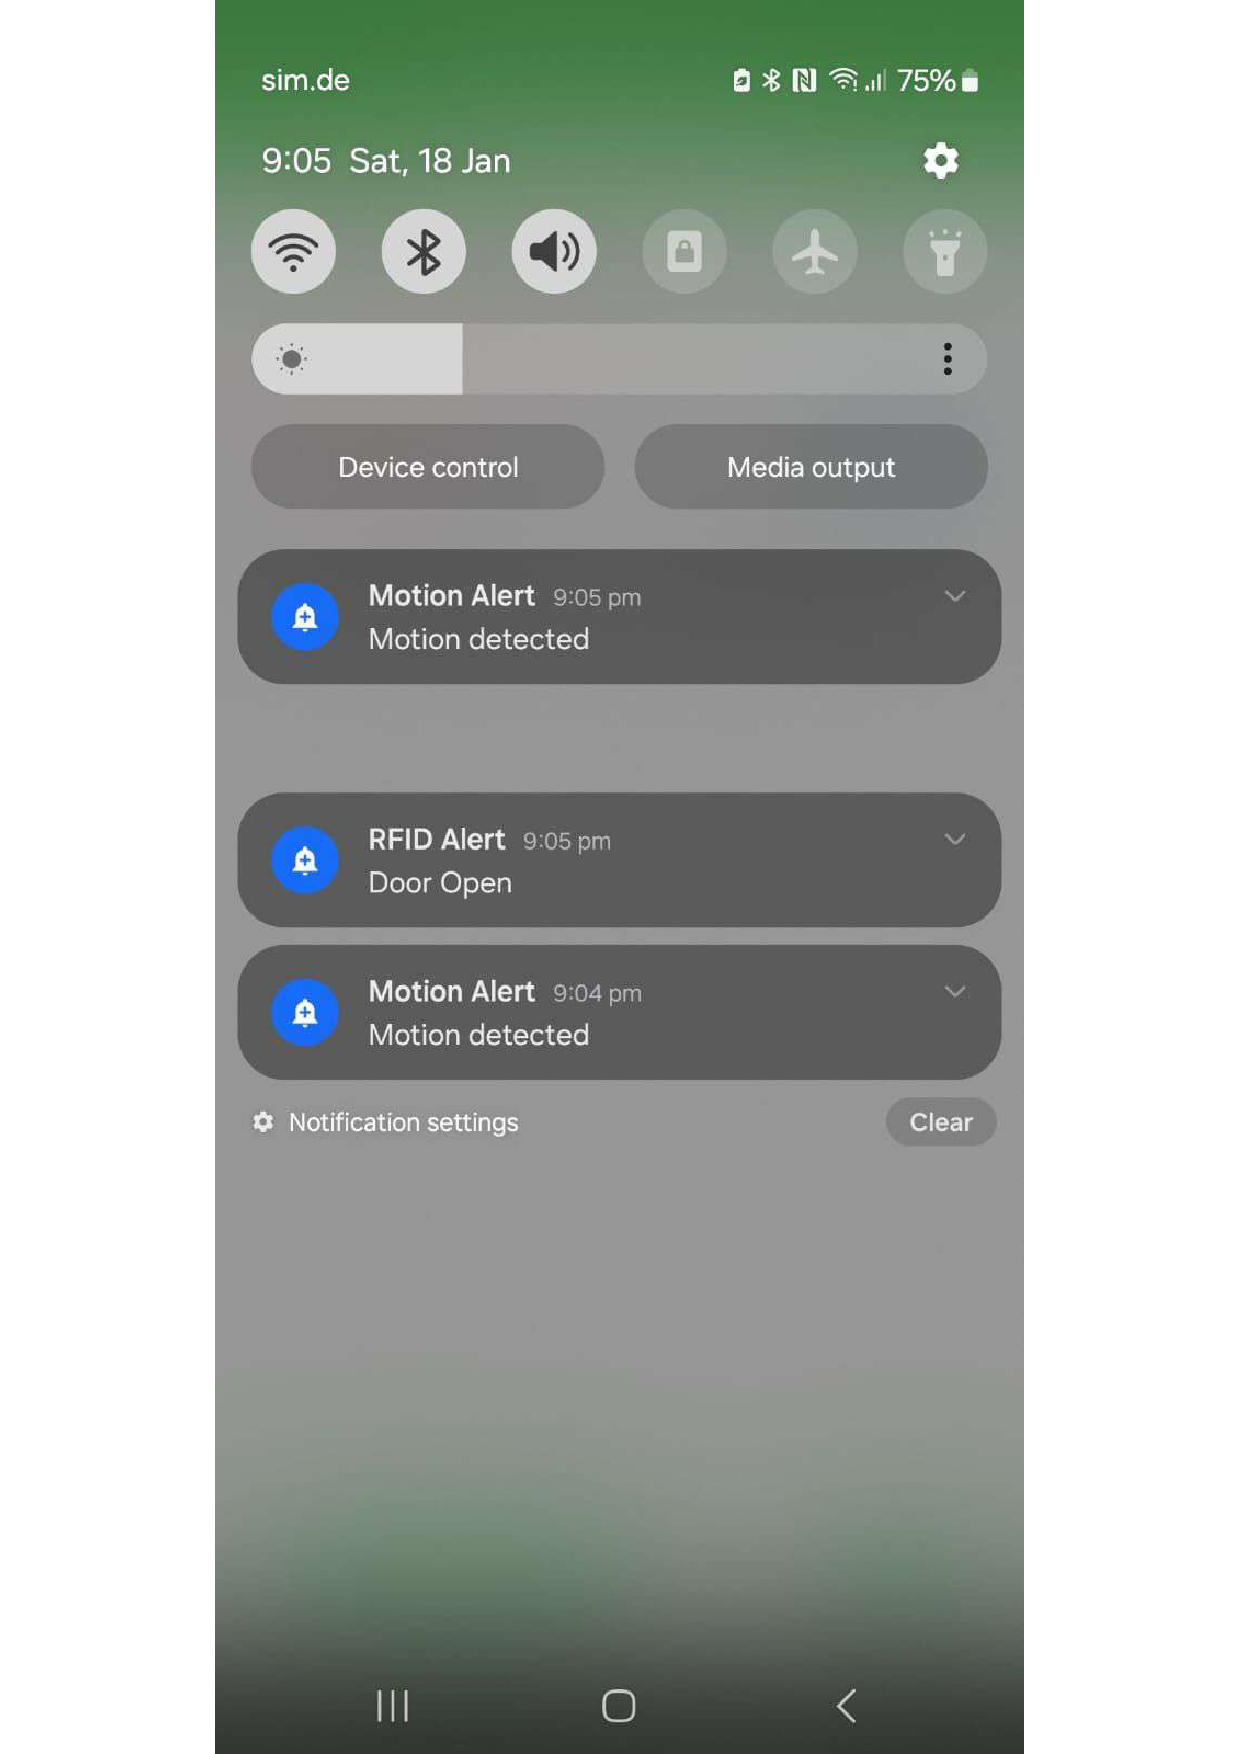
\includegraphics[width=0.9\textwidth]{notification.pdf}
        \caption{Notification alert for motion detection or RFID scan}
        \label{fig:notification}
    \end{minipage}
    
    \vspace{0.7cm} % Increase spacing between rows
\end{figure}



\begin{figure}[h]
    \centering
    

    \begin{minipage}{0.45\textwidth}
        \centering
        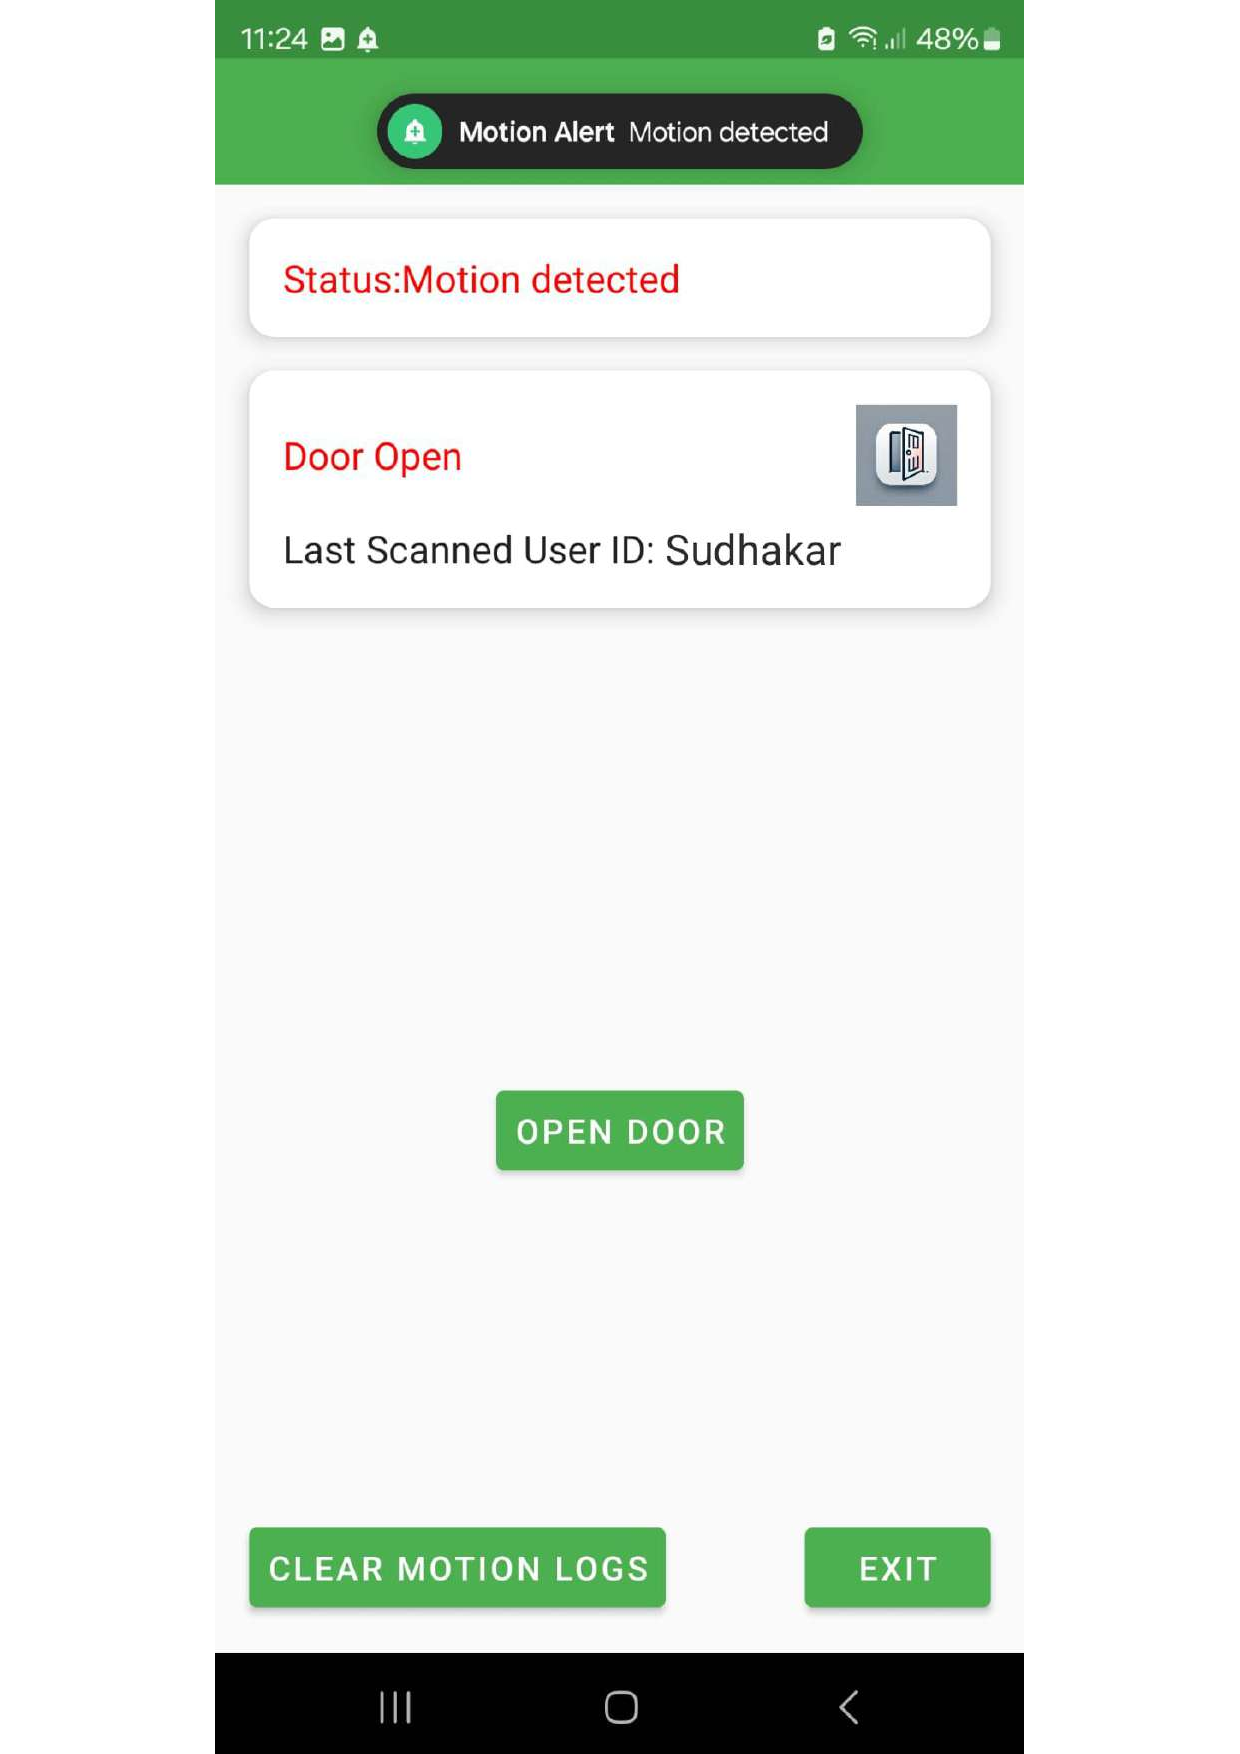
\includegraphics[width=0.9\textwidth]{user.pdf}
        \caption{Valid user unlocking the door with an authorized RFID tag}
        \label{fig:user}
    \end{minipage}
    \hfill
    \begin{minipage}{0.45\textwidth}
        \centering
        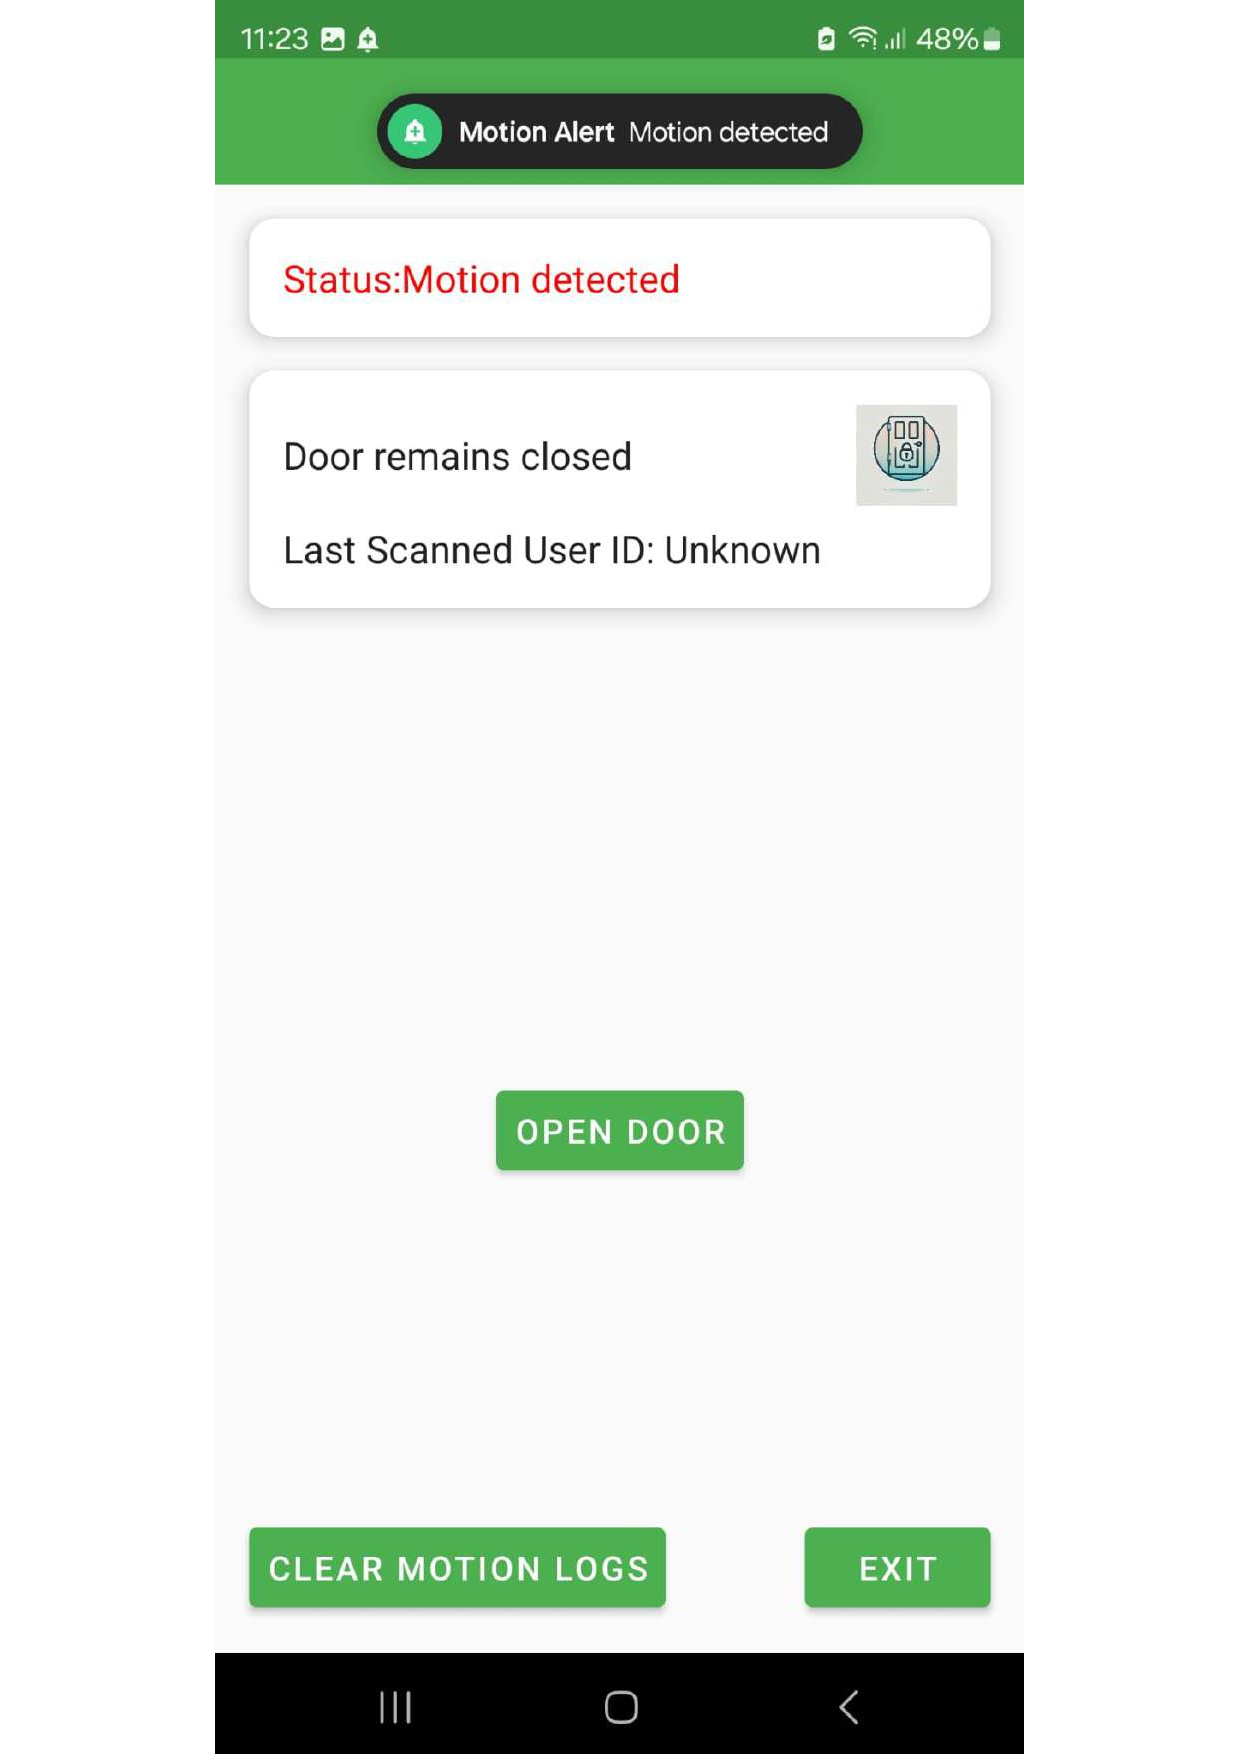
\includegraphics[width=0.9\textwidth]{unknown.pdf}
        \caption{Unauthorized access attempt using an unregistered RFID tag}
        \label{fig:unknown}
    \end{minipage}
\end{figure}





\section{Discussion}
\label{sec:discussion} 
The Smart Security Door Lock System enhances home security by integrating embedded systems, wireless communication, and a mobile application. This part will address the research
questions we previously posed, provide a brief explanation of the difficulties encountered
throughout the development phase, and examine any constraints.

\subsection{Challenges}
The Smart Security Door Lock System had a few significant problems to overcome when it came to coding. The biggest was the EM-18 RFID reader, which sends data out on its TX pin, and had to be correctly connected to the RX pin of the PineCone BL602 in order to receive data. The EM-18 operates at 9600 bps, but the PineCone's default UART speed is 2 Mbps, so configuring the multiple UARTs at different speeds was an issue. Another important step was ensuring that the selection pin on the EM-18 was set correctly to enable UART communication instead of Wiegand protocol.

Second, it was difficult to regulate the servo motor with PWM signals because it needed precise angles to lock and unlock the door properly. The final difficulty was making the Wi-Fi, motion sensor, and EM-18 RFID reader work at the same time. The system needed to execute various tasks without delays or conflicts. The motion sensor had to detect movement without interfering with the RFID reader's data transmission. The Wi-Fi module had to stay connected and responsive while the rest of the system was running. All these elements had to be balanced seamlessly and required careful task scheduling and efficient UART and PWM settings. All these issues aside, the system was integrated successfully with the right TX-RX connections, UART settings, and sensor coordination.
\subsection{Research Question Solutions}
Let’s now explore the research questions. We have addressed each of the four study
questions that were previously mentioned in the report in section~\ref{sec:questions}.
\subsubsection{Integration of Wi-Fi, Motion Sensor, and RFID Authentication}
To integrate Wi-Fi, a motion sensor, and RFID authentication without causing delays or conflicts, the system employs FreeRTOS-based task scheduling to efficiently manage multiple processes on the PineCone BL602 microcontroller. By assigning different priorities to tasks, real-time authentication and motion detection can operate smoothly without interference. The system optimizes data transfer using buffered UART communication, ensuring low-latency responses while preventing conflicts between connected peripherals.
\subsubsection{Benefits of a Mobile App in Smart Door Lock Systems}
The mobile application improves security with remote access control, real-time alert, and monitoring of access logs. Users can remotely open doors, receive instant alerts for invalid attempts, and remotely view security logs. The application improves the overall user experience by simplifying security management and eliminating the physical key factor. It is also a single point to track door activity and motion detection.

\subsubsection{Efficient Management of Multiple UART Devices}
Managing multiple UART devices on a resource-limited microcontroller requires precise synchronization of baud rates and buffering techniques. The system configures UART peripherals with interrupt-driven communication to prevent data loss and collisions. By allocating dedicated RX/TX pins for each device and implementing a FIFO buffer, the system ensures stable and error-free data transfer between the RFID reader, Wi-Fi module, and motion sensor.
\subsubsection{Impact of Motion Detection on Security}
Motion detection significantly improves security with real-time alert of suspicious movement near the door. PIR motion detection is not dependent on RFID authentication and detects movement to trigger the mobile app alert. The additional layer of security detects potential threat, reduces false alarms, and blocks unauthorized entry even when RFID authentication has been taken over. Motion-activated alerts provide round-the-clock monitoring, enhancing the security of the system.

\subsection{Limitations}

Our project also has certain limitations due to the hardware constraints of the PineCone BL602 microcontroller. One of its major limitations is its small memory capacity, where it has 276KB SRAM and 2MB embedded flash memory. While the SRAM is reserved for runtime activity, the flash memory holds firmware and other data, which takes up the available space for RFID tag information storage. This constraint makes the storage of large numbers of authenticated RFID tags problematic, making the system less suitable for applications where there is extensive user authentication required. The system also relies on Wi-Fi to enable the control of the motion sensor and EM-18 RFID reader to be run concurrently. However, due to the PineCone BL602's weak processing power, the addition of other peripherals or sensors can burden the system and lead to potential performance loss. The second constraint is the limited support to attach more than one mobile application to the Wi-Fi module at once. The system is restricted in accepting a single mobile device interacting with it and therefore restricts multi-user activity and reduces versatility in community spaces. These limitations necessitate further enhancement in terms of memory enhancement, addition of external storage, and improved support for connectivity in order to improve the scalability and performance of the system.
\section{Future Work}
\label{sec:future}

Although the Smart Security Door Lock System has been successfully implemented, there is still room for improvement and upgrading. One of the significant upgrades is the incorporation of multi-factor authentication (MFA) using both biometric authentication (fingerprint or face recognition) and RFID authentication for greater security. This will prevent unauthorized access even when the RFID tag is cloned or lost \cite{Shirali2023}. Modern MFA systems, such as those offered by Duo Security, reinforce the necessity of multiple verification layers for smart door locks by adding additional security steps and reducing vulnerabilities \cite{DuoMFA2025}.

Cloud-based access control is another area where the system can be improved. The system now runs on a local network and only allows remote access within the same Wi-Fi connection. Incorporating a cloud-based system would enable users to check access logs and unlock the door from anywhere in the world. Secure cloud authentication protocols such as OAuth 2.0 or blockchain-based authentication could also add an extra layer of security and prevent unauthorized break-ins \cite{Shirali2023}.

Other than that, power optimization is also among the most important areas of future work. The system is currently reliant on a stable power supply, but the utilization of low-power communication protocols such as LoRaWAN (Long Range Wide Area Network) or BLE (Bluetooth Low Energy) can enable battery-powered operation, making the system viable for regions with no direct power supply connection. These protocols are able to conserve energy, making the system operational for extended periods on battery \cite{LoRaLock2022}.

Finally, anomaly detection may be performed using machine learning in order to detect suspicious access patterns or motion sensor activity. A model of AI can learn normal user behavior and flag or lock the system in the event of a probable security breach \cite{Tiwari2024}.

By implementing these enhancements, the Smart Security Door Lock System can evolve into a more secure, scalable, and intelligent access control solution.


\section{Conclusion }
\label{sec:conclusion}
The Smart Security Door Lock System combines RFID authentication, motion sensing, Wi-Fi, and smartphone app-based distance monitoring solely for security and ease of use. The implementation of IoT technology and hybrid systems makes the project an actual, scalable, and affordable solution to traditional lock systems. The system effectively averts security threats by blocking intruders, sending real-time alarms, and enabling remote control via a simple smartphone app.

Through rigorous testing, the system was found to provide fast authentication, real-time movement detection, and secure Wi-Fi data communication, ensuring maximum performance. However, certain limitations, such as the requirement of a local network, single-device connectivity, and memory constraints, highlight areas for future improvement. Future-proofed enhancements will be feasible in fields such as multi-factor authentication (MFA), cloud-based remote access, low-power communication protocols, and anomaly detection based on artificial intelligence, enhancing both security and usability.

This research highlights the potential of IoT in future-proofing access control systems, demonstrating that smart door locks are at the core of security, surveillance, and automation for residential and commercial applications. With continued expansion and enhancement of its capabilities, the Smart Security Door Lock System can evolve into an AI-powered automated security solution, serving as a foundation for future home security technologies within the IoT ecosystem.

% Show cited references
	\printbibliography[title={References}]



% Table 5: Review Remarks
\begin{longtable}{|l|p{4cm}|p{3cm}|p{4cm}|} % Adjust column widths as needed
    \caption{Review Remarks} % Caption for the table
    \label{tab:review_remarks} \\ % Label for referencing the table
    \hline
    \textbf{Reviewer} & \textbf{Review} & \textbf{Decision} & \textbf{Remark} \\ % Column headers
    \hline
    \endfirsthead % Header for the first page
    \hline
    \textbf{Reviewer} & \textbf{Review} & \textbf{Decision} & \textbf{Remark} \\ % Column headers for subsequent pages
    \hline
    \endhead % Header for subsequent pages
    \hline
    \endfoot % Footer for all pages
    \hline
    \endlastfoot % Footer for the last page

    % Table content
    Reviewer & The paper covers IoT-based security solutions but does not highlight unique contributions explicitly. & Accepted & Please refer to section~\ref{sec:intro} \\
    \hline
    Reviewer & Some sections were repetitive (e.g., motion detection). Refining language and structure will improve readability. & Accepted & Improved language and structure \\
    \hline
    Reviewer & The system lacks advanced innovations like biometric integration or AI-enhanced security. & Reject & section~\ref{sec:future}: Future Work (Biometric integration and AI-enhanced security can be suggested as future work). \\
    \hline
    Reviewer & Include quantifiable performance metrics (e.g., system latency, reliability, power consumption). & Accepted & Please refer to section~\ref{sec:results} (Quantitative metrics like response time and power consumption are included). \\
    \hline
    Reviewer & Include more professional diagrams with clear labeling to enhance understanding of hardware and software integration. & Accepted & Please refer to Figures in section~\ref{sec:implementation} and section~\ref{sec:results} (Diagrams were improved with clear labeling). \\
    \hline
    Reviewer & Address grammatical inconsistencies and improve overall language quality for a more professional presentation. & Accepted & Throughout the Document (Language and grammar were improved). \\
    \hline
    Reviewer & Enhance the mobile app functionality by adding features for remote access, real-time monitoring, and comprehensive user feedback mechanisms. & Accepted & The app already supports remote access and real-time monitoring via Wi-Fi(refer section~\ref{sec:testing}) See section~\ref{sec:future} for future enhancements. \\
    \hline
    Reviewer & Improve clarity in the methodology section, particularly the circuit design and software integration. & Accepted & Please refer to section~\ref{sec:implementation} (Explained circuit design and software integration) \\
    \hline
    Reviewer & Include usability test results or user feedback to bring in a sense of realism regarding usability. & Accepted & Usability testing was conducted to enhance realism and reliability. \\
    \hline
    Reviewer & The abstract is verbose and contains redundant statements. Refine it for conciseness and clarity. & Accepted & Abstract (The abstract was refined for conciseness and clarity). \\
    \hline
    Reviewer & Address potential cybersecurity risks and mitigations for IoT systems. & Accepted & Please refer to section~\ref{sec:discussion} \\
    \hline
    Reviewer & Develop a clear roadmap to address current limitations, including debugging challenges and sensor integration issues. & Accepted & Please refer to section~\ref{sec:discussion} \\
    \hline
    Reviewer & Improve the motion sensor’s reliability to minimize false positives and ensure consistent and accurate detection. & Accepted & Please refer to section~\ref{sec:implementation} \\
    \hline
    Reviewer & Some sections, such as "Hardware Integration," contain technical details that could be better structured for readability. & Accepted & Please refer to section~\ref{sec:implementation} \\
    \hline
    Reviewer & The conclusion could be more impactful by summarizing key findings and emphasizing the system’s contributions. & Accepted & Please refer to section~\ref{sec:conclusion} \\
    \hline
    Reviewer & The energy efficiency discussion is minimal. More details on power consumption and optimization should be included. & Accepted & Please refer to section~\ref{sec:results} \\
    \hline
    Reviewer & The literature review mentions various studies individually, but there could be more synthesis of findings. & Accepted & Please refer to section~\ref{sec:review} \\
    \hline
    Reviewer & Some results are only described qualitatively; showing images would make them more understandable. & Accepted & Please refer to section~\ref{sec:results} \\
    \hline
    Reviewer & Future work should explore alternative security mechanisms, such as blockchain-based authentication. & Accepted & Please refer to section~\ref{sec:future} (Blockchain-based authentication was suggested as future work). \\
    \hline
    Reviewer & The introduction should better define the scope and objectives of the study. & Accepted & Please refer to section~\ref{sec:intro} \\
    \hline
    Reviewer & Consider discussing potential failure modes of the system and how to mitigate them. & Accepted & Please refer to section~\ref{sec:discussion} \\
    \hline
    Reviewer & The testing methodology should be more detailed, describing how the system was evaluated in real-world conditions. & Accepted & Refer to section~\ref{sec:methodology}, section~\ref{sec:implementation}, and section~\ref{sec:results} \\
    \hline
    Reviewer & More references should be added to support claims about RFID limitations and motion detection challenges. & Accepted & Additional references were added for RFID and motion detection \\
    \hline
\end{longtable}

    
\end{document}
